\documentclass[9pt, landscape, a4paper,twosided]{extarticle}

\newcommand{\universityName}{University of Dhaka}
\newcommand{\teamName}{DU\_Scolps}
\newcommand{\firstMember}{Asif Jawad}
\newcommand{\secondMember}{Sakib Hassan}
\newcommand{\thirdMember}{Bholanath Das Niloy}
\newcommand{\contestName}{NCPC 2024}
\newcommand{\updateDate}{February 2024}

\usepackage{minted}
%\usemintedstyle{bw}
\usepackage{sectsty}
\usepackage{fouriernc}
\usepackage[T1]{fontenc}
\usepackage{framed}
\usepackage{makeidx}
\usepackage{enumitem}
\usepackage{titlesec}
\usepackage[scaled=0.9]{DejaVu Sans Mono}
\usepackage[utf8]{inputenc}
\usepackage[english]{babel}
\usepackage{listings}
\usepackage{amsmath}
\usepackage{verbatim}
\usepackage{hyperref}
\usepackage[dvipsnames]{xcolor}
\usepackage{multicol}
\usepackage{geometry}
\usepackage{amssymb,tikz,psfrag,epstopdf}
\geometry{verbose,landscape,a4paper,tmargin=1.25cm,bmargin=0cm,lmargin=0.75cm,rmargin=.25cm}

\newcommand{\maketeampage}{
	\pagestyle{empty}
	\setcounter{page}{0}
	\begin{center}
		\strut % Magic
		\vspace{2cm}\\
		
\includegraphics[width=3cm]{logo}\\
		\vspace{0.5cm}
		{\fontsize{24}{30} \fontfamily{lmss} \selectfont {\universityName}\\}
		\vspace{2cm}
		{\fontsize{60}{60} \fontfamily{lmss} \selectfont {\teamName}\\}
		\vspace{1cm}
		{\fontsize{24}{30} \fontfamily{lmss} \selectfont { {\firstMember}, {\secondMember}, {\thirdMember} }\\}
		\vspace{2cm}
		{\fontsize{24}{30} \fontfamily{lmss} \selectfont {Team Reference Document for {\contestName}}}\\
		\vspace{1cm}
		{\fontsize{18}{24} \fontfamily{lmss} \selectfont {Updated: {\updateDate}}}\\
		\vspace{1cm}
	\end{center}
	\clearpage
	\pagestyle{fancy}
}

\newcommand{\printdescription}[1]{
  \codeheader{Description}{#1}
}
\newcommand{\printusage}[1]{
  \codeheader{Usage}{\texttt{#1}}
}
\newcommand{\printtime}[1]{
  \codeheader{Time}{#1}
}
\newcommand{\printmemory}[1]{
  \codeheader{Memory}{#1}
}
\newcommand{\codeheader}[2]{
	{\par\noindent\normalsize{\textbf{#1:} #2\par}}
}
\newcommand{\bigo}[1] {\ensuremath{\mathcal{O} \left( #1 \right)}}

\newenvironment{myitemize}
{ \begin{itemize}[leftmargin=.5cm]
    \setlength{\itemsep}{0pt}
    \setlength{\parskip}{0pt}
    \setlength{\parsep}{0pt}     }
{ \end{itemize}                  }

\setlength{\parindent}{0pt}
\newcommand*{\Scale}[2][4]{\scalebox{#1}{$#2$}}%

\setlength{\columnsep}{1.5mm}
\setlength{\columnseprule}{1px}

\setcounter{secnumdepth}{4}
\setcounter{tocdepth}{4}

\BeforeBeginEnvironment{minted}{\vspace{0mm}}
\AfterEndEnvironment{minted}{\vspace{-1mm}}

\linespread{0.18}
\usepackage{fancyhdr}
\pagestyle{fancy}
\fancyhf{}
\renewcommand{\headrulewidth}{1pt}
% \renewcommand{\footrulewidth}{1pt}
\renewcommand{\theFancyVerbLine}{\sffamily \textcolor[rgb]{0.15,0.15,0.15}{\small \arabic{FancyVerbLine}}}
%\rfoot{\thepage}

\lhead{\textcolor{MidnightBlue}{\textit{\textbf{\universityName}}} | \textcolor{MidnightBlue}{\textit{\textbf{\teamName}}}}
\setlength\headheight{16pt}
\rhead{\thepage}
\headsep = 0pt
% \textheight = 7.75in
\textheight = 7.95in
% \footskip = 16pt
\footskip = 0mm

\titlespacing*{\section}{0pt}{0}{0}
\titlespacing*{\subsection}{0pt}{0}{0}
\titlespacing*{\subsubsection}{0pt}{0}{0}

\titleformat{\section}
  {\normalfont\fontsize{10}{15}\bfseries}{\thesection}{1em}{}
\titleformat{\subsection}
  {\normalfont\fontsize{8}{15}\bfseries}{\thesubsection}{1em}{}
\titleformat{\subsubsection}
  {\normalfont\fontsize{8}{15}\bfseries}{\thesubsubsection}{1em}{}
\subsectionfont{\Huge}

\begin{document}
\maketeampage
\begin{multicols*}{3}
\tableofcontents
\vspace{2mm}
% \noindent\makebox[\linewidth]{\rule{\paperwidth}{0.4pt}}
\noindent\rule{9.7cm}{1pt}
\vspace{2mm}\section{DP}
\subsection{CHT}
\begin{minted}[
    breaklines = true,
    breakanywhere = true,
    frame=lines,    
    fontfamily=tt,
    linenos=false,
    numberblanklines=true,
    numbersep=2pt,
    gobble=0,
    framerule=1pt,
    framesep=1mm,
    funcnamehighlighting=true,
    tabsize=1,
    obeytabs=false,
    mathescape=false
    samepage=false, %with this setting you can force the list to appear on the same page
    showspaces=false,
    showtabs =false,
    texcl=false
]{C++}

ll M[MAX] , C[MAX];

struct CHT {
  int len , cur;
  void init() {
    len = 0 ,cur = 0;
  }

  inline bool isBad(ll nm,ll nc) {
    return ( (C[len-1]-C[len-2])/(double)(M[len-2]-M[len-1]) >= (nc-C[len-2])/(double)(M[len-2]-nm) );
    //return ( (C[len-1]-C[len-2])*(M[len-2]-nm) >= (M[len-2]-M[len-1])*(nc-C[len-2]) );
  }

  inline void addLine(ll nm,ll nc) {
    if(len == 0) M[len] = nm , C[len] = nc , ++len;
    else if( M[len-1] == nm ) {
      if(C[len-1] <= nc) return;
      else C[len-1] = nc;
    }
    else {
      while(len >= 2 && isBad(nm,nc)) --len;
      M[len] = nm , C[len] = nc , ++len;
    }
  }

  inline ll getY(int id , ll x) {
    return ( M[id]*x + C[id] );
  }

  inline ll sortedQuery( ll x ) {
    if(cur >= len ) cur = len-1;
    while( cur < len-1 && getY(cur+1,x) >= getY(cur,x) ) cur++;
    return getY(cur,x);
  }

  inline ll TS( ll x ) {
    int low = 0, high = len-1 , mid ;
    while( high - low > 1 ) {
      mid = low + high >> 1;
      if(getY(mid,x) < getY(mid+1,x)) low = mid + 1;
      else high = mid;
    }
    return max(getY(low,x),getY(high,x));
  }
};

CHT cht;
cht.init();
\end{minted}

\subsection{DC\_Optimization}
\begin{minted}[
    breaklines = true,
    breakanywhere = true,
    frame=lines,    
    fontfamily=tt,
    linenos=false,
    numberblanklines=true,
    numbersep=2pt,
    gobble=0,
    framerule=1pt,
    framesep=1mm,
    funcnamehighlighting=true,
    tabsize=1,
    obeytabs=false,
    mathescape=false
    samepage=false, %with this setting you can force the list to appear on the same page
    showspaces=false,
    showtabs =false,
    texcl=false
]{C++}

void compute(int L, int R, int optL, int optR){
  if(L > R) return;
  int M = L + R >> 1;
  pair<ll, int> best(1LL << 60, -1);
  for(int k = optL; k <= min(M, optR); k++){
    best = min(best, {dp[prv][k] + C[k + 1][M], k});
  }
  dp[now][M] = best.ff;
  compute(L, M - 1, optL, best.ss);
  compute(M + 1, R, best.ss, optR);
}
\end{minted}

\subsection{SOS\_DP}
\begin{minted}[
    breaklines = true,
    breakanywhere = true,
    frame=lines,    
    fontfamily=tt,
    linenos=false,
    numberblanklines=true,
    numbersep=2pt,
    gobble=0,
    framerule=1pt,
    framesep=1mm,
    funcnamehighlighting=true,
    tabsize=1,
    obeytabs=false,
    mathescape=false
    samepage=false, %with this setting you can force the list to appear on the same page
    showspaces=false,
    showtabs =false,
    texcl=false
]{C++}

for(int mask = 0; mask < (1<<N); ++mask){
        dp[mask][-1] = A[mask];
        for(int i = 0;i < N; ++i){
            if(mask & (1<<i)) dp[mask][i] = dp[mask][i-1] + dp[mask ^ (1<<i)][i-1];
            else dp[mask][i] = dp[mask][i-1];
        }
        F[mask] = dp[mask][N-1];
    }
    for(int i = 0; i<(1<<N); ++i) F[i] = A[i];
    for(int i = 0;i < N; ++i)
        for(int mask = 0; mask < (1<<N); ++mask){
            if(mask & (1<<i))
                F[mask] += F[mask^(1<<i)];
        }
\end{minted}

\subsection{dynamic\_cht}
\begin{minted}[
    breaklines = true,
    breakanywhere = true,
    frame=lines,    
    fontfamily=tt,
    linenos=false,
    numberblanklines=true,
    numbersep=2pt,
    gobble=0,
    framerule=1pt,
    framesep=1mm,
    funcnamehighlighting=true,
    tabsize=1,
    obeytabs=false,
    mathescape=false
    samepage=false, %with this setting you can force the list to appear on the same page
    showspaces=false,
    showtabs =false,
    texcl=false
]{C++}

//add lines with -m and -b and return -ans to
//make this code work for minimums.(not -x)
const ll inf = -(1LL << 62);
struct line {
  ll m, b;
  mutable function<const line*() > succ;
  bool operator < (const line& rhs) const {
    if (rhs.b != inf) return m < rhs.m;
    const line* s = succ();
    if (!s) return 0;
    ll x = rhs.m;
    return b - s->b < (s->m - m) * x;
  }
};
struct CHT : public multiset<line> {
  bool bad(iterator y) {
    auto z = next(y);
    if (y == begin()) {
      if (z == end()) return 0;
      return y -> m == z -> m && y -> b <= z -> b;
    }
    auto x = prev(y);
    if (z == end()) return y -> m == x -> m && y -> b <= x -> b;
    return 1.0 * (x -> b - y -> b) * (z -> m - y -> m) >= 1.0 * (y -> b - z -> b) * (y -> m - x -> m);
  }
  void add(ll m, ll b) {
    auto y = insert({ m, b });
    y->succ = [ = ] { return next(y) == end() ? 0 : &*next(y); };
    if (bad(y)) {
      erase(y);
      return;
    }
    while (next(y) != end() && bad(next(y))) erase(next(y));
    while (y != begin() && bad(prev(y))) erase(prev(y));
  }
  ll query(ll x) {
    auto l = *lower_bound((line) {
      x, inf
    });
    return l.m * x + l.b;
  }
};
CHT* cht;
ll a[N], b[N];
int32_t main() {
  ios_base::sync_with_stdio(0);
  cin.tie(0);

  int n;
  cin >> n;
  for(int i = 0; i < n; i++) cin >> a[i];
  for(int i = 0; i < n; i++) cin >> b[i];
  cht = new CHT();
  cht -> add(-b[0], 0);
  ll ans = 0;
  for(int i = 1; i < n; i++) {
    ans = -cht -> query(a[i]);
    cht -> add(-b[i], -ans);
  }
  cout << ans << nl;
  return 0;
}
\end{minted}

\section{Data_Structure}
\subsection{2D\_segtree}
\begin{minted}[
    breaklines = true,
    breakanywhere = true,
    frame=lines,    
    fontfamily=tt,
    linenos=false,
    numberblanklines=true,
    numbersep=2pt,
    gobble=0,
    framerule=1pt,
    framesep=1mm,
    funcnamehighlighting=true,
    tabsize=1,
    obeytabs=false,
    mathescape=false
    samepage=false, %with this setting you can force the list to appear on the same page
    showspaces=false,
    showtabs =false,
    texcl=false
]{C++}

struct Point {
    int x, y, mx;
    Point() {}
    Point(int x, int y, int mx) : x(x), y(y), mx(mx) {}

    bool operator < (const Point& other) const {
        return mx < other.mx;
    }
};

struct Segtree2d {

    // I didn't calculate the exact size needed in terms of 2D container size.
    // If anyone, please edit the answer.
    // It's just a safe size to store nodes for MAX * MAX 2D grids which won't cause stack overflow :)
    Point T[500000]; // TODO: calculate the accurate space needed

    int n, m;

    // initialize and construct segment tree
    void init(int n, int m) {
        this -> n = n;
        this -> m = m;
        build(1, 1, 1, n, m);
    }

    // build a 2D segment tree from data [ (a1, b1), (a2, b2) ]
    // Time: O(n logn)
    Point build(int node, int a1, int b1, int a2, int b2) {
        // out of range
        if (a1 > a2 or b1 > b2)
            return def();

        // if it is only a single index, assign value to node
        if (a1 == a2 and b1 == b2)
            return T[node] = Point(a1, b1, P[a1][b1]);

        // split the tree into four segments
        T[node] = def();
        T[node] = maxNode(T[node], build(4 * node - 2, a1, b1, (a1 + a2) / 2, (b1 + b2) / 2 ) );
        T[node] = maxNode(T[node], build(4 * node - 1, (a1 + a2) / 2 + 1, b1, a2, (b1 + b2) / 2 ));
        T[node] = maxNode(T[node], build(4 * node + 0, a1, (b1 + b2) / 2 + 1, (a1 + a2) / 2, b2) );
        T[node] = maxNode(T[node], build(4 * node + 1, (a1 + a2) / 2 + 1, (b1 + b2) / 2 + 1, a2, b2) );
        return T[node];
    }

    // helper function for query(int, int, int, int);
    Point query(int node, int a1, int b1, int a2, int b2, int x1, int y1, int x2, int y2) {
        // if we out of range, return dummy
        if (x1 > a2 or y1 > b2 or x2 < a1 or y2 < b1 or a1 > a2 or b1 > b2)
            return def();

        // if it is within range, return the node
        if (x1 <= a1 and y1 <= b1 and a2 <= x2 and b2 <= y2)
            return T[node];

        // split into four segments
        Point mx = def();
        mx = maxNode(mx, query(4 * node - 2, a1, b1, (a1 + a2) / 2, (b1 + b2) / 2, x1, y1, x2, y2) );
        mx = maxNode(mx, query(4 * node - 1, (a1 + a2) / 2 + 1, b1, a2, (b1 + b2) / 2, x1, y1, x2, y2) );
        mx = maxNode(mx, query(4 * node + 0, a1, (b1 + b2) / 2 + 1, (a1 + a2) / 2, b2, x1, y1, x2, y2) );
        mx = maxNode(mx, query(4 * node + 1, (a1 + a2) / 2 + 1, (b1 + b2) / 2 + 1, a2, b2, x1, y1, x2, y2));

        // return the maximum value
        return mx;
    }

    // query from range [ (x1, y1), (x2, y2) ]
    // Time: O(logn)
    Point query(int x1, int y1, int x2, int y2) {
        return query(1, 1, 1, n, m, x1, y1, x2, y2);
    }

    // helper function for update(int, int, int);
    Point update(int node, int a1, int b1, int a2, int b2, int x, int y, int value) {
        if (a1 > a2 or b1 > b2)
            return def();

        if (x > a2 or y > b2 or x < a1 or y < b1)
            return T[node];

        if (x == a1 and y == b1 and x == a2 and y == b2)
            return T[node] = Point(x, y, value);

        Point mx = def();
        mx = maxNode(mx, update(4 * node - 2, a1, b1, (a1 + a2) / 2, (b1 + b2) / 2, x, y, value) );
        mx = maxNode(mx, update(4 * node - 1, (a1 + a2) / 2 + 1, b1, a2, (b1 + b2) / 2, x, y, value));
        mx = maxNode(mx, update(4 * node + 0, a1, (b1 + b2) / 2 + 1, (a1 + a2) / 2, b2, x, y, value));
        mx = maxNode(mx, update(4 * node + 1, (a1 + a2) / 2 + 1, (b1 + b2) / 2 + 1, a2, b2, x, y, value) );
        return T[node] = mx;
    }

    // update the value of (x, y) index to 'value'
    // Time: O(logn)
    Point update(int x, int y, int value) {
        return update(1, 1, 1, n, m, x, y, value);
    }

    // utility functions; these functions are virtual because they will be overridden in child class
    virtual Point maxNode(Point a, Point b) {
        return max(a, b);
    }

    // dummy node
    virtual Point def() {
        return Point(0, 0, -INF);
    }
};

/* 2D Segment Tree for range minimum query; a override of Segtree2d class */
struct Segtree2dMin : Segtree2d {
    // overload maxNode() function to return minimum value
    Point maxNode(Point a, Point b) {
        return min(a, b);
    }

    Point def() {
        return Point(0, 0, INF);
    }
};
\end{minted}

\subsection{Segtree\_beats\_desc}
\begin{minted}[
    breaklines = true,
    breakanywhere = true,
    frame=lines,    
    fontfamily=tt,
    linenos=false,
    numberblanklines=true,
    numbersep=2pt,
    gobble=0,
    framerule=1pt,
    framesep=1mm,
    funcnamehighlighting=true,
    tabsize=1,
    obeytabs=false,
    mathescape=false
    samepage=false, %with this setting you can force the list to appear on the same page
    showspaces=false,
    showtabs =false,
    texcl=false
]{C++}

/*
Description: For update Ai → Ai mod x and similar, keep range min,
max in node and lazily update whenever min = max. For update
Ai → min(Ai, x) and similar, keep range max, second max in node and
lazily update whenever x > second max.
Time: O(log^2 N), (log N)
 */
\end{minted}

\subsection{gp\_hash\_table}
\begin{minted}[
    breaklines = true,
    breakanywhere = true,
    frame=lines,    
    fontfamily=tt,
    linenos=false,
    numberblanklines=true,
    numbersep=2pt,
    gobble=0,
    framerule=1pt,
    framesep=1mm,
    funcnamehighlighting=true,
    tabsize=1,
    obeytabs=false,
    mathescape=false
    samepage=false, %with this setting you can force the list to appear on the same page
    showspaces=false,
    showtabs =false,
    texcl=false
]{C++}

using namespace __gnu_pbds;
const int RANDOM = chrono::high_resolution_clock::now().time_since_epoch().count();
using namespace __gnu_pbds;
struct chash {
  const int RANDOM = (long long)(make_unique<char>().get()) ^ chrono::high_resolution_clock::now().time_since_epoch().count();
  static unsigned long long hash_f(unsigned long long x) {
    x += 0x9e3779b97f4a7c15;
    x = (x ^ (x >> 30)) * 0xbf58476d1ce4e5b9;
    x = (x ^ (x >> 27)) * 0x94d049bb133111eb;
    return x ^ (x >> 31);
  }
  static unsigned hash_combine(unsigned a, unsigned b) { return a * 31 + b; }
  ll operator()(ll x) const { return hash_f(x)^RANDOM; }
};
gp_hash_table<key, long long, chash> table;
\end{minted}

\subsection{iterative\_segtree}
\begin{minted}[
    breaklines = true,
    breakanywhere = true,
    frame=lines,    
    fontfamily=tt,
    linenos=false,
    numberblanklines=true,
    numbersep=2pt,
    gobble=0,
    framerule=1pt,
    framesep=1mm,
    funcnamehighlighting=true,
    tabsize=1,
    obeytabs=false,
    mathescape=false
    samepage=false, %with this setting you can force the list to appear on the same page
    showspaces=false,
    showtabs =false,
    texcl=false
]{C++}

const int N = 500010;
int n, a[N], tree[N << 1];
void init() {
    for (int i = 0; i < n; ++i) tree[n + i] = a[i];
    for (int i = n - 1; i >= 0; --i) {
        tree[i] = min(tree[i << 1], tree[i << 1 | 1]);
    }
}
void update(int p, int v) {
    for (tree[p += n] = v; p > 1; p >>= 1) {
        tree[p >> 1] = min(tree[p], tree[p ^ 1]);
    }
}
int query(int l, int r) {
    int ret = INT_MAX;
    for (l += n, r += n; l < r; l >>= 1, r >>= 1) {
        if (l & 1) ret = min(ret, tree[l++]);
        if (r & 1) ret = min(ret, tree[--r]);
    }
    return ret;
}
\end{minted}

\subsection{mos\_algo}
\begin{minted}[
    breaklines = true,
    breakanywhere = true,
    frame=lines,    
    fontfamily=tt,
    linenos=false,
    numberblanklines=true,
    numbersep=2pt,
    gobble=0,
    framerule=1pt,
    framesep=1mm,
    funcnamehighlighting=true,
    tabsize=1,
    obeytabs=false,
    mathescape=false
    samepage=false, %with this setting you can force the list to appear on the same page
    showspaces=false,
    showtabs =false,
    texcl=false
]{C++}

struct data{
  int l, r, id, bn;
  data() {}
  data(int _l, int _r, int _id){
    l = _l, r = _r, id = _id;
    bn = l / block_sz;
  }
  bool operator < (const data& other) const{
    if (bn != other.bn) return (bn < other.bn);
    return ((bn & 1) ? (r < other.r) : (r > other.r));
  }

}

int curL = 0, curR = -1;
for(int i = 0; i < Q.sz; i++){
  while(curL > Q[i].L){
    curL--; add(curL);
  }
  while(curR < Q[i].R){
    curR++; add(curR);
  }
  while(curL < Q[i].L){
    remove(curL); curL++;
  }
  while(curR > Q[i].R){
    remove(curR); curR--;
  }
}
\end{minted}

\subsection{ordered\_set}
\begin{minted}[
    breaklines = true,
    breakanywhere = true,
    frame=lines,    
    fontfamily=tt,
    linenos=false,
    numberblanklines=true,
    numbersep=2pt,
    gobble=0,
    framerule=1pt,
    framesep=1mm,
    funcnamehighlighting=true,
    tabsize=1,
    obeytabs=false,
    mathescape=false
    samepage=false, %with this setting you can force the list to appear on the same page
    showspaces=false,
    showtabs =false,
    texcl=false
]{C++}

using namespace std;
using namespace __gnu_pbds;
typedef tree<
    int ,
    null_type ,
    less < int > , // "less_equal<int>," for multiset
    rb_tree_tag,
    tree_order_statistics_node_update > ordered_set;
ordered_set OS;
\end{minted}

\subsection{persistant\_segtree}
\begin{minted}[
    breaklines = true,
    breakanywhere = true,
    frame=lines,    
    fontfamily=tt,
    linenos=false,
    numberblanklines=true,
    numbersep=2pt,
    gobble=0,
    framerule=1pt,
    framesep=1mm,
    funcnamehighlighting=true,
    tabsize=1,
    obeytabs=false,
    mathescape=false
    samepage=false, %with this setting you can force the list to appear on the same page
    showspaces=false,
    showtabs =false,
    texcl=false
]{C++}

const int MAX = 100010;

int ncnt = 0;

struct node {
  int sum;
  int left,right;
  node() {}
  node(int val) {
    sum = val;
    left = right = -1;
  }
} tree[ ? ];

int ara[MAX];
int version[MAX];

void build(int n,int st,int ed) {
  if (st==ed) {
    tree[n] = node(ara[st]);
    return;
  }

  int mid = (st+ed) / 2;

  tree[n].left = ++ncnt;
  tree[n].right = ++ncnt;

  build(tree[n].left, st, mid);
  build(tree[n].right, mid+1, ed);

  tree[n].sum = tree[tree[n].left].sum + tree[tree[n].right].sum;
}

void update(int prev,int cur,int st,int ed,int id, int val)
{
  if (id > ed or id < st) return;
  if (st == ed) {
    tree[cur] = node(val);
    return;
  }
  int mid = (st+ed) / 2;
  if (id <= mid) {
    tree[cur].right = tree[prev].right;
    tree[cur].left = ++ncnt;
    update(tree[prev].left,tree[cur].left, st, mid, id, val);
  }
  else {
    tree[cur].left = tree[prev].left;
    tree[cur].right = ++ncnt;
    update(tree[prev].right, tree[cur].right, mid+1, ed, id, val);
  }
  tree[cur].sum = tree[tree[cur].left].sum + tree[tree[cur].right].sum;
}

int query(int n,int st,int ed,int i,int j){
  if(st>=i && ed<=j) return tree[n].sum;
  int mid = (st+ed)/2;
  if(mid<i) return query(tree[n].right,mid+1,ed,i,j);
  else if(mid>=j) return query(tree[n].left,st,mid,i,j);
  else return query(tree[n].left,st,mid,i,j) + query(tree[n].right,mid+1,ed,i,j);
}

int main() {
  int n,q,l,r,k;

  sii(n,q);

  version[0] = ++ncnt;
  build(version[0],1,n);

  version[1] = ++ncnt;
  update(version[0],version[1],1,n,id,val);

  query(version[0],1,n,id,id);
  query(version[1],1,n,id,id);

  return 0;
}
\end{minted}

\subsection{segment\_tree}
\begin{minted}[
    breaklines = true,
    breakanywhere = true,
    frame=lines,    
    fontfamily=tt,
    linenos=false,
    numberblanklines=true,
    numbersep=2pt,
    gobble=0,
    framerule=1pt,
    framesep=1mm,
    funcnamehighlighting=true,
    tabsize=1,
    obeytabs=false,
    mathescape=false
    samepage=false, %with this setting you can force the list to appear on the same page
    showspaces=false,
    showtabs =false,
    texcl=false
]{C++}

int ara[MAX];

struct node {
  int sum;
} tree[4 * MAX];

int lazy[4 * MAX];

node Merge(node a, node b) {
  node ret;
  ret.sum = a.sum + b.sum;
  return ret;
}

void lazyUpdate(int n, int st, int ed) {
  if(lazy[n] != 0){
    tree[n].sum += ((ed - st + 1) * lazy[n]);
    if(st != ed){
      lazy[2 * n] += lazy[n];
      lazy[2 * n + 1] += lazy[n];
    }
    lazy[n] = 0;
  }
}

void build(int n, int st, int ed) {
  lazy[n] = 0;
  if(st == ed){
    tree[n].sum = ara[st];
    return;
  }
  int mid = (st + ed) / 2;
  build(2 * n, st, mid);
  build(2 * n + 1, mid + 1, ed);
  tree[n] = Merge(tree[2 * n], tree[2 * n + 1]);
}

void update(int n, int st, int ed, int i, int j, int v) {
  lazyUpdate(n, st, ed);
  if(st > j or ed < i) return;
  if(st >= i and ed <= j){
    lazy[n] += v;
    lazyUpdate(n, st, ed);
    return;
  }
  int mid = (st + ed) / 2;
  update(2 * n, st, mid, i, j, v);
  update(2 * n + 1, mid+1, ed, i, j, v);
  tree[n] = Merge(tree[2 * n], tree[2 * n + 1]);
}

node query(int n, int st, int ed, int i, int j) {
  lazyUpdate(n, st, ed);
  if(st >= i and ed <= j) return tree[n];
  int mid = (st + ed) / 2;
  if(mid < i) return query(2 * n + 1, mid + 1, ed, i, j);
  else if(mid >= j) return query(2 * n, st, mid, i, j);
  else return Merge(query(2 * n, st, mid, i, j), query(2 * n + 1, mid + 1, ed, i, j));
}
\end{minted}

\subsection{sparse\_table}
\begin{minted}[
    breaklines = true,
    breakanywhere = true,
    frame=lines,    
    fontfamily=tt,
    linenos=false,
    numberblanklines=true,
    numbersep=2pt,
    gobble=0,
    framerule=1pt,
    framesep=1mm,
    funcnamehighlighting=true,
    tabsize=1,
    obeytabs=false,
    mathescape=false
    samepage=false, %with this setting you can force the list to appear on the same page
    showspaces=false,
    showtabs =false,
    texcl=false
]{C++}

int st[K + 1][MAXN];
void build() {
  std::copy(array.begin(), array.end(), st[0]);
  for (int i = 1; i <= K; i++)
    for (int j = 0; j + (1 << i) <= N; j++)
      st[i][j] = f(st[i - 1][j], st[i - 1][j + (1 << (i - 1))]);
}
\end{minted}

\section{Geometry}
\subsection{2D Primitive}
\subsubsection{Angle}
A class for ordering angles (as represented by int points and a number of rotations around the origin). Useful for rotational sweeping.
Sometimes also represents points or vectors.
\begin{minted}[breaklines = true,
    breakanywhere = true,
    frame=lines,    
    fontfamily=tt,
    linenos=false,
    numberblanklines=true,
    numbersep=2pt,
    gobble=0,
    framerule=1pt,
    framesep=1mm,
    funcnamehighlighting=true,
    tabsize=1,
    obeytabs=false,
    mathescape=false
    samepage=false, %with this setting you can force the list to appear on the same page
    showspaces=false,
    showtabs =false,
    texcl=false]{C++}
/* Usage:
 *  vector<Angle> v = {w[0], w[0].t360() ...}; // sorted
 *  int j = 0; rep(i,0,n) { while (v[j] < v[i].t180()) ++j; }
 *  // sweeps j such that (j-i) represents the number of positively oriented triangles with vertices at 0 and i
*/
struct Angle {
  int x, y;
  int t;
  Angle(int x, int y, int t=0) : x(x), y(y), t(t) {}
  Angle operator-(Angle b) const { return {x-b.x, y-b.y, t}; }
  int half() const {
    assert(x || y);
    return y < 0 || (y == 0 && x < 0);
  }
  Angle t90() const { return {-y, x, t + (half() && x >= 0)}; }
  Angle t180() const { return {-x, -y, t + half()}; }
  Angle t360() const { return {x, y, t + 1}; }
};
bool operator<(Angle a, Angle b) {
  // add a.dist2() and b.dist2() to also compare distances
  return make_tuple(a.t, a.half(), a.y * (ll)b.x) < make_tuple(b.t, b.half(), a.x * (ll)b.y);
}

// Given two points, this calculates the smallest angle between
// them, i.e., the angle that covers the defined line segment.
pair<Angle, Angle> segmentAngles(Angle a, Angle b) {
  if (b < a) swap(a, b);
  return (b < a.t180() ? make_pair(a, b) : make_pair(b, a.t360()));
}
Angle operator+(Angle a, Angle b) { // point a + vector b
  Angle r(a.x + b.x, a.y + b.y, a.t);
  if (a.t180() < r) r.t--;
  return r.t180() < a ? r.t360() : r;
}
Angle angleDiff(Angle a, Angle b) { // angle b - angle a
  int tu = b.t - a.t; a.t = b.t;
  return {a.x*b.x + a.y*b.y, a.x*b.y - a.y*b.x, tu - (b < a)};
}
\end{minted}

\subsubsection{Line Distance}
\begin{minipage}{75mm}
Returns the signed distance between point p and the line containing points a and b. Positive value on left side and negative on right as seen from a towards b. a==b gives nan. P is supposed to be Point<T> or Point3D<T> where T is e.g. double or long long. It uses products in intermediate steps so watch out for overflow if using int or long long. Using Point3D will always give a non-negative distance. For Point3D, call .dist on the result of the cross product.
\end{minipage}
\begin{minipage}{15mm}
\includegraphics[width=\textwidth]{"../code/Geometry/2D Primitive/lineDistance"}
\end{minipage}
\begin{minted}[breaklines = true,
    breakanywhere = true,
    frame=lines,    
    fontfamily=tt,
    linenos=false,
    numberblanklines=true,
    numbersep=2pt,
    gobble=0,
    framerule=1pt,
    framesep=1mm,
    funcnamehighlighting=true,
    tabsize=1,
    obeytabs=false,
    mathescape=false
    samepage=false, %with this setting you can force the list to appear on the same page
    showspaces=false,
    showtabs =false,
    texcl=false]{C++}
#include "Point.h"

template<class P>
double lineDist(const P& a, const P& b, const P& p) {
  return (double)(b-a).cross(p-a)/(b-a).dist();
}
\end{minted}

\subsubsection{Line Intersection}
\begin{minipage}{75mm}
If a unique intersection point of the lines going through s1,e1 and s2,e2 exists \{1, point\} is returned.
If no intersection point exists \{0, (0,0)\} is returned and if infinitely many exists \{-1, (0,0)\} is returned.
The wrong position will be returned if P is Point<ll> and the intersection point does not have integer coordinates.
Products of three coordinates are used in intermediate steps so watch out for overflow if using int or ll.
\end{minipage}
\begin{minipage}{15mm}
\includegraphics[width=\textwidth]{"../code/Geometry/2D Primitive/lineIntersection"}
\end{minipage}
\begin{minted}[breaklines = true,
    breakanywhere = true,
    frame=lines,    
    fontfamily=tt,
    linenos=false,
    numberblanklines=true,
    numbersep=2pt,
    gobble=0,
    framerule=1pt,
    framesep=1mm,
    funcnamehighlighting=true,
    tabsize=1,
    obeytabs=false,
    mathescape=false
    samepage=false, %with this setting you can force the list to appear on the same page
    showspaces=false,
    showtabs =false,
    texcl=false]{C++}
/* Usage:
 *  auto res = lineInter(s1,e1,s2,e2);
 *  if (res.first == 1)
 *    cout << "intersection point at " << res.second << endl;
 */
#pragma once

#include "Point.h"

template<class P>
pair<int, P> lineInter(P s1, P e1, P s2, P e2) {
  auto d = (e1 - s1).cross(e2 - s2);
  if (d == 0) // if parallel
    return {-(s1.cross(e1, s2) == 0), P(0, 0)};
  auto p = s2.cross(e1, e2), q = s2.cross(e2, s1);
  return {1, (s1 * p + e1 * q) / d};
}
\end{minted}

\subsubsection{Linear Transformation}
\begin{minipage}{75mm}
Apply the linear transformation (translation, rotation and scaling) which takes line p0-p1 to line q0-q1 to point r.
\end{minipage}
\begin{minipage}{15mm}
\vspace{-8mm}
\includegraphics[width=\textwidth]{"../code/Geometry/2D Primitive/linearTransformation"}
\vspace{-2mm}
\end{minipage}
\begin{minted}[breaklines = true,
    breakanywhere = true,
    frame=lines,    
    fontfamily=tt,
    linenos=false,
    numberblanklines=true,
    numbersep=2pt,
    gobble=0,
    framerule=1pt,
    framesep=1mm,
    funcnamehighlighting=true,
    tabsize=1,
    obeytabs=false,
    mathescape=false
    samepage=false, %with this setting you can force the list to appear on the same page
    showspaces=false,
    showtabs =false,
    texcl=false]{C++}
#include "Point.h"

typedef Point<double> P;
P linearTransformation(const P& p0, const P& p1, const P& q0, const P& q1, const P& r) {
  P dp = p1-p0, dq = q1-q0, num(dp.cross(dq), dp.dot(dq));
  return q0 + P((r-p0).cross(num), (r-p0).dot(num))/dp.dist2();
}
\end{minted}

\subsubsection{On Segment}
\begin{minted}{C++}
/* Description: Returns true iff p lies on the line segment from s to e.
 * Use \texttt{(segDist(s,e,p)<=epsilon)} instead when using Point<double>.
 */
#include "Point.h"

template<class P> bool onSegment(P s, P e, P p) {
  return p.cross(s, e) == 0 && (s - p).dot(e - p) <= 0;
}
\end{minted}
\subsubsection{Point Sort}
\begin{minted}[
    breaklines = true,
    breakanywhere = true,
    frame=lines,    
    fontfamily=tt,
    linenos=false,
    numberblanklines=true,
    numbersep=2pt,
    gobble=0,
    framerule=1pt,
    framesep=1mm,
    funcnamehighlighting=true,
    tabsize=1,
    obeytabs=false,
    mathescape=false
    samepage=false, %with this setting you can force the list to appear on the same page
    showspaces=false,
    showtabs =false,
    texcl=false
]{C++}

// sort the points in counterclockwise order that starts from the half line x≤0,y=0.

using namespace std;

typedef long long ll;
typedef pair <ll, ll> point;

#define x first
#define y second

int main() {
  int n; cin >> n;
  vector <point> p(n);
  for (auto &it : p) scanf("%lld %lld", &it.x, &it.y);
  sort(p.begin(), p.end(), [] (point a, point b) {
    return atan2l(a.y, a.x) < atan2l(b.y, b.x);
  });
  for (auto it : p) printf("%lld %lld\n", it.x, it.y);
  return 0;
}
\end{minted}

\subsubsection{Point}
\begin{minted}[
    breaklines = true,
    breakanywhere = true,
    frame=lines,    
    fontfamily=tt,
    linenos=false,
    numberblanklines=true,
    numbersep=2pt,
    gobble=0,
    framerule=1pt,
    framesep=1mm,
    funcnamehighlighting=true,
    tabsize=1,
    obeytabs=false,
    mathescape=false
    samepage=false, %with this setting you can force the list to appear on the same page
    showspaces=false,
    showtabs =false,
    texcl=false
]{C++}

// Class to handle points in the plane. T can be e.g. double or long long. (Avoid int.)
template <class T> int sgn(T x) { return (x > 0) - (x < 0); }
template<class T>
struct Point {
	typedef Point P;
	T x, y;
	explicit Point(T x=0, T y=0) : x(x), y(y) {}
	bool operator<(P p) const { return tie(x,y) < tie(p.x,p.y); }
	bool operator==(P p) const { return tie(x,y)==tie(p.x,p.y); }
	P operator+(P p) const { return P(x+p.x, y+p.y); }
	P operator-(P p) const { return P(x-p.x, y-p.y); }
	P operator*(T d) const { return P(x*d, y*d); }
	P operator/(T d) const { return P(x/d, y/d); }
	T dot(P p) const { return x*p.x + y*p.y; }
	T cross(P p) const { return x*p.y - y*p.x; }
	T cross(P a, P b) const { return (a-*this).cross(b-*this); }
	T dist2() const { return x*x + y*y; }
	double dist() const { return sqrt((double)dist2()); }
	// angle to x-axis in interval [-pi, pi]
	double angle() const { return atan2(y, x); }
	P unit() const { return *this/dist(); } // makes dist()=1
	P perp() const { return P(-y, x); } // rotates +90 degrees
	P normal() const { return perp().unit(); }
	// returns point rotated 'a' radians ccw around the origin
	P rotate(double a) const {
		return P(x*cos(a)-y*sin(a),x*sin(a)+y*cos(a)); }
	friend ostream& operator<<(ostream& os, P p) {
		return os << "(" << p.x << "," << p.y << ")"; }
};
\end{minted}

\subsubsection{Segment Distance}
\begin{minipage}{75mm}
Returns the shortest distance between point p and the line segment from point s to e.
\end{minipage}
\begin{minipage}{15mm}
\vspace{-10mm}
\includegraphics[width=\textwidth]{"../code/Geometry/2D Primitive/SegmentDistance"}
\end{minipage}
\begin{minted}[breaklines = true,
    breakanywhere = true,
    frame=lines,    
    fontfamily=tt,
    linenos=false,
    numberblanklines=true,
    numbersep=2pt,
    gobble=0,
    framerule=1pt,
    framesep=1mm,
    funcnamehighlighting=true,
    tabsize=1,
    obeytabs=false,
    mathescape=false
    samepage=false, %with this setting you can force the list to appear on the same page
    showspaces=false,
    showtabs =false,
    texcl=false]{C++}
/* Usage: 
 *  Point<double> a, b(2,2), p(1,1);
 *  bool onSegment = segDist(a,b,p) < 1e-10;
 * Status: tested
 */
#pragma once

#include "Point.h"

typedef Point<double> P;
double segDist(P& s, P& e, P& p) {
  if (s==e) return (p-s).dist();
  auto d = (e-s).dist2(), t = min(d,max(.0,(p-s).dot(e-s)));
  return ((p-s)*d-(e-s)*t).dist()/d;
}

\end{minted}

\subsubsection{Segment Intersection}
\begin{minipage}{75mm}
If a unique intersection point between the line segments going from s1 to e1 and from s2 to e2 exists then it is returned.
If no intersection point exists an empty vector is returned. If infinitely many exist a vector with 2 elements is returned, containing the endpoints of the common line segment.
The wrong position will be returned if P is Point<ll> and the intersection point does not have integer coordinates.
Products of three coordinates are used in intermediate steps so watch out for overflow if using int or long long.
\end{minipage}
\begin{minipage}{15mm}
\includegraphics[width=\textwidth]{"../code/Geometry/2D Primitive/SegmentIntersection"}
\end{minipage}
\begin{minted}[breaklines = true,
    breakanywhere = true,
    frame=lines,    
    fontfamily=tt,
    linenos=false,
    numberblanklines=true,
    numbersep=2pt,
    gobble=0,
    framerule=1pt,
    framesep=1mm,
    funcnamehighlighting=true,
    tabsize=1,
    obeytabs=false,
    mathescape=false
    samepage=false, %with this setting you can force the list to appear on the same page
    showspaces=false,
    showtabs =false,
    texcl=false]{C++}
/* Usage:
 * vector<P> inter = segInter(s1,e1,s2,e2);
 * if (sz(inter)==1)
 *   cout << "segments intersect at " << inter[0] << endl;
 * Status: stress-tested, tested on kattis:intersection
 */

#include "Point.h"
#include "OnSegment.h"

template<class P> vector<P> segInter(P a, P b, P c, P d) {
  auto oa = c.cross(d, a), ob = c.cross(d, b),
       oc = a.cross(b, c), od = a.cross(b, d);
  // Checks if intersection is single non-endpoint point.
  if (sgn(oa) * sgn(ob) < 0 && sgn(oc) * sgn(od) < 0)
    return {(a * ob - b * oa) / (ob - oa)};
  set<P> s;
  if (onSegment(c, d, a)) s.insert(a);
  if (onSegment(c, d, b)) s.insert(b);
  if (onSegment(a, b, c)) s.insert(c);
  if (onSegment(a, b, d)) s.insert(d);
  return {all(s)};
}
\end{minted}

\subsubsection{Side Of}
Returns where $p$ is as seen from $s$ towards $e$. 1/0/-1 $\Leftrightarrow$ left/on line/right. If the optional argument $eps$ is given 0 is returned if $p$ is within distance $eps$ from the line. P is supposed to be Point<T> where T is e.g. double or long long. It uses products in intermediate steps so watch out for overflow if using int or long long.
\begin{minted}{C++}
/* Usage:
 *  bool left = sideOf(p1,p2,q)==1;
 * Status: tested
 */
#include "Point.h"

template<class P>
int sideOf(P s, P e, P p) { return sgn(s.cross(e, p)); }

template<class P>
int sideOf(const P& s, const P& e, const P& p, double eps) {
  auto a = (e-s).cross(p-s);
  double l = (e-s).dist()*eps;
  return (a > l) - (a < -l);
}
\end{minted}
\subsection{3D}
\subsubsection{3D Convex Hull}
\begin{minted}[
    breaklines = true,
    breakanywhere = true,
    frame=lines,    
    fontfamily=tt,
    linenos=false,
    numberblanklines=true,
    numbersep=2pt,
    gobble=0,
    framerule=1pt,
    framesep=1mm,
    funcnamehighlighting=true,
    tabsize=1,
    obeytabs=false,
    mathescape=false
    samepage=false, %with this setting you can force the list to appear on the same page
    showspaces=false,
    showtabs =false,
    texcl=false
]{C++}

#define ll long long
#define sz(x) ((int) (x).size())
#define all(x) (x).begin(), (x).end()
#define vi vector<int>
#define pii pair<int, int>
#define rep(i, a, b) for(int i = (a); i < (b); i++)
using namespace std;
template<typename T>
using minpq = priority_queue<T, vector<T>, greater<T>>;

typedef long double ftype;

struct pt3 {
  ftype x, y, z;
  pt3(ftype x = 0, ftype y = 0, ftype z = 0) : x(x), y(y), z(z) {}
  pt3 operator-(const pt3 &o) const {
    return pt3(x - o.x, y - o.y, z - o.z);
  }
  pt3 cross(const pt3 &o) const {
    return pt3(y * o.z - z * o.y, z * o.x - x * o.z, x * o.y - y * o.x);
  }
  ftype dot(const pt3 &o) const {
    return x * o.x + y * o.y + z * o.z;
  }
};

// A face is represented by the indices of its three points a, b, c.
// It also stores an outward-facing normal vector q
struct face {
  int a, b, c;
  pt3 q;
};

// modify this depending on the coordinate sizes in your use case
const ftype EPS = 1e-9;

vector<face> hull3(const vector<pt3> &p) {
  int n = sz(p);
  assert(n >= 3);
  vector<face> f;

  // Consider an edge (a->b) dead if it is not a CCW edge of some current face
  // If an edge is alive but not its reverse, this is an exposed edge.
  // We should add new faces on the exposed edges.
  vector<vector<bool>> dead(n, vector<bool>(n, true));
  auto add_face = [&](int a, int b, int c) {
    f.push_back({a, b, c, (p[b] - p[a]).cross(p[c] - p[a])});
    dead[a][b] = dead[b][c] = dead[c][a] = false;
  };

  // Initialize the convex hull of the first 3 points as a
  // triangular disk with two faces of opposite orientation
  add_face(0, 1, 2);
  add_face(0, 2, 1);
  rep(i, 3, n) {
    // f2 will be the list of faces invisible to the added point p[i]
    vector<face> f2;
    for(face &F : f) {
      if((p[i] - p[F.a]).dot(F.q) > EPS) {
        // this face is visible to the new point, so mark its edges as dead
        dead[F.a][F.b] = dead[F.b][F.c] = dead[F.c][F.a] = true;
      }else {
        f2.push_back(F);
      }
    }
    // Add a new face for each exposed edge.
    // Only check edges of alive faces for being exposed.
    f.clear();
    for(face &F : f2) {
      int arr[3] = {F.a, F.b, F.c};
      rep(j, 0, 3) {
        int a = arr[j], b = arr[(j + 1) % 3];
        if(dead[b][a]) {
          add_face(b, a, i);
        }
      }
    }
    f.insert(f.end(), all(f2));
  }
  return f;
}
\end{minted}

\subsubsection{Point3D}
Class to handle points in 3D space.T can be e.g. double or long long.
\begin{minted}{C++}
template<class T> struct Point3D {
  typedef Point3D P;
  typedef const P& R;
  T x, y, z;
  explicit Point3D(T x=0, T y=0, T z=0) : x(x), y(y), z(z) {}
  bool operator<(R p) const {
    return tie(x, y, z) < tie(p.x, p.y, p.z); }
  bool operator==(R p) const {
    return tie(x, y, z) == tie(p.x, p.y, p.z); }
  P operator+(R p) const { return P(x+p.x, y+p.y, z+p.z); }
  P operator-(R p) const { return P(x-p.x, y-p.y, z-p.z); }
  P operator*(T d) const { return P(x*d, y*d, z*d); }
  P operator/(T d) const { return P(x/d, y/d, z/d); }
  T dot(R p) const { return x*p.x + y*p.y + z*p.z; }
  P cross(R p) const {
    return P(y*p.z - z*p.y, z*p.x - x*p.z, x*p.y - y*p.x);
  }
  T dist2() const { return x*x + y*y + z*z; }
  double dist() const { return sqrt((double)dist2()); }
  //Azimuthal angle (longitude) to x-axis in interval [-pi, pi]
  double phi() const { return atan2(y, x); } 
  //Zenith angle (latitude) to the z-axis in interval [0, pi]
  double theta() const { return atan2(sqrt(x*x+y*y),z); }
  P unit() const { return *this/(T)dist(); } //makes dist()=1
  //returns unit vector normal to *this and p
  P normal(P p) const { return cross(p).unit(); }
  //returns point rotated 'angle' radians ccw around axis
  P rotate(double angle, P axis) const {
    double s = sin(angle), c = cos(angle); P u = axis.unit();
    return u*dot(u)*(1-c) + (*this)*c - cross(u)*s;
  }
};
\end{minted}

\subsubsection{Polyhedron Volume}
Description: Magic formula for the volume of a polyhedron. Faces should point outwards.
\begin{minted}[breaklines = true,
    breakanywhere = true,
    frame=lines,    
    fontfamily=tt,
    linenos=false,
    numberblanklines=true,
    numbersep=2pt,
    gobble=0,
    framerule=1pt,
    framesep=1mm,
    funcnamehighlighting=true,
    tabsize=1,
    obeytabs=false,
    mathescape=false
    samepage=false, %with this setting you can force the list to appear on the same page
    showspaces=false,
    showtabs =false,
    texcl=false]{C++}
template<class V, class L>
double signedPolyVolume(const V& p, const L& trilist) {
  double v = 0;
  for (auto i : trilist) v += p[i.a].cross(p[i.b]).dot(p[i.c]);
  return v / 6;
}
\end{minted}

\subsubsection{Spherical Distance}
Returns the shortest distance on the sphere with radius radius between the points with azimuthal angles (longitude) f1 ($\phi_1$) and f2 ($\phi_2$) from x axis and zenith angles (latitude) t1 ($\theta_1$) and t2 ($\theta_2$) from z axis (0 = north pole). All angles measured in radians. The algorithm starts by converting the spherical coordinates to cartesian coordinates so if that is what you have you can use only the two last rows. dx*radius is then the difference between the two points in the x direction and d*radius is the total distance between the points.
\begin{minted}{C++}
double sphericalDistance(double f1, double t1,
    double f2, double t2, double radius) {
  double dx = sin(t2)*cos(f2) - sin(t1)*cos(f1);
  double dy = sin(t2)*sin(f2) - sin(t1)*sin(f1);
  double dz = cos(t2) - cos(t1);
  double d = sqrt(dx*dx + dy*dy + dz*dz);
  return radius*2*asin(d/2);
}
\end{minted}

\subsection{Circle}
\subsubsection{Circle Intersection}
Computes the pair of points at which two circles intersect. Returns false in case of no intersection.
\begin{minted}{C++}
#include "Point.h"

typedef Point<double> P;
bool circleInter(P a,P b,double r1,double r2,pair<P, P>* out) {
  if (a == b) { assert(r1 != r2); return false; }
  P vec = b - a;
  double d2 = vec.dist2(), sum = r1+r2, dif = r1-r2,
         p = (d2 + r1*r1 - r2*r2)/(d2*2), h2 = r1*r1 - p*p*d2;
  if (sum*sum < d2 || dif*dif > d2) return false;
  P mid = a + vec*p, per = vec.perp() * sqrt(fmax(0, h2) / d2);
  *out = {mid + per, mid - per};
  return true;
}
\end{minted}
\subsubsection{Circle Polygon Intersection}
Returns the area of the intersection of a circle with a ccw polygon. \\
Time: $O(n)$
\begin{minted}{C++}
#include "Point.h"

typedef Point<double> P;
#define arg(p, q) atan2(p.cross(q), p.dot(q))
double circlePoly(P c, double r, vector<P> ps) {
  auto tri = [&](P p, P q) {
    auto r2 = r * r / 2;
    P d = q - p;
    auto a = d.dot(p)/d.dist2(), b = (p.dist2()-r*r)/d.dist2();
    auto det = a * a - b;
    if (det <= 0) return arg(p, q) * r2;
    auto s = max(0., -a-sqrt(det)), t = min(1., -a+sqrt(det));
    if (t < 0 || 1 <= s) return arg(p, q) * r2;
    P u = p + d * s, v = p + d * t;
    return arg(p,u) * r2 + u.cross(v)/2 + arg(v,q) * r2;
  };
  auto sum = 0.0;
  rep(i,0,sz(ps))
    sum += tri(ps[i] - c, ps[(i + 1) % sz(ps)] - c);
  return sum;
}
\end{minted}
\subsubsection{Circle Tangents}
Finds the external tangents of two circles, or internal if r2 is negated.
Can return 0, 1, or 2 tangents -- 0 if one circle contains the other (or overlaps it, in the internal case, or if the circles are the same);
1 if the circles are tangent to each other (in which case .first = .second and the tangent line is perpendicular to the line between the centers).
.first and .second give the tangency points at circle 1 and 2 respectively.
To find the tangents of a circle with a point set r2 to 0.
\begin{minted}{C++}
#include "Point.h"

template<class P>
vector<pair<P, P>> tangents(P c1, double r1, P c2, double r2) {
  P d = c2 - c1;
  double dr = r1 - r2, d2 = d.dist2(), h2 = d2 - dr * dr;
  if (d2 == 0 || h2 < 0)  return {};
  vector<pair<P, P>> out;
  for (double sign : {-1, 1}) {
    P v = (d * dr + d.perp() * sqrt(h2) * sign) / d2;
    out.push_back({c1 + v * r1, c2 + v * r2});
  }
  if (h2 == 0) out.pop_back();
  return out;
}
\end{minted}
\subsubsection{CircumCircle}
\begin{minipage}{75mm}
The circumcirle of a triangle is the circle intersecting all three vertices. ccRadius returns the radius of the circle going through points A, B and C and ccCenter returns the center of the same circle.
\end{minipage}
\begin{minipage}{15mm}
\vspace{-2mm}
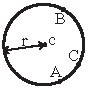
\includegraphics[width=\textwidth]{../code/Geometry/Circle/circumcircle}
\end{minipage}
\begin{minted}[breaklines = true,
    breakanywhere = true,
    frame=lines,    
    fontfamily=tt,
    linenos=false,
    numberblanklines=true,
    numbersep=2pt,
    gobble=0,
    framerule=1pt,
    framesep=1mm,
    funcnamehighlighting=true,
    tabsize=1,
    obeytabs=false,
    mathescape=false
    samepage=false, %with this setting you can force the list to appear on the same page
    showspaces=false,
    showtabs =false,
    texcl=false]{C++}
#include "Point.h"

typedef Point<double> P;
double ccRadius(const P& A, const P& B, const P& C) {
  return (B-A).dist()*(C-B).dist()*(A-C).dist()/
      abs((B-A).cross(C-A))/2;
}
P ccCenter(const P& A, const P& B, const P& C) {
  P b = C-A, c = B-A;
  return A + (b*c.dist2()-c*b.dist2()).perp()/b.cross(c)/2;
}
\end{minted}

\subsection{Polygon}
\subsubsection{Hull Diameter}
Returns the two points with max distance on a convex hull (ccw, no duplicate/collinear points).
\begin{minted}[breaklines = true,
    breakanywhere = true,
    frame=lines,    
    fontfamily=tt,
    linenos=false,
    numberblanklines=true,
    numbersep=2pt,
    gobble=0,
    framerule=1pt,
    framesep=1mm,
    funcnamehighlighting=true,
    tabsize=1,
    obeytabs=false,
    mathescape=false
    samepage=false, %with this setting you can force the list to appear on the same page
    showspaces=false,
    showtabs =false,
    texcl=false]{C++}
#include "Point.h"

typedef Point<ll> P;
array<P, 2> hullDiameter(vector<P> S) {
  int n = sz(S), j = n < 2 ? 0 : 1;
  pair<ll, array<P, 2>> res({0, {S[0], S[0]}});
  rep(i,0,j)
    for (;; j = (j + 1) % n) {
      res = max(res, {(S[i] - S[j]).dist2(), {S[i], S[j]}});
      if ((S[(j + 1) % n] - S[j]).cross(S[i + 1] - S[i]) >= 0)
        break;
    }
  return res.second;
}

\end{minted}

\subsubsection{Line Hull Intersection}
Line-convex polygon intersection. The polygon must be ccw and have no collinear points.
lineHull(line, poly) returns a pair describing the intersection of a line with the polygon:
\begin{itemize*}
\item $(-1, -1)$ if no collision,
\item $(i, -1)$ if touching the corner $i$,
\item $(i, i)$ if along side $(i, i+1)$,
\item $(i, j)$ if crossing sides $(i, i+1)$ and $(j, j+1)$.
\end{itemize*}
In the last case, if a corner $i$ is crossed, this is treated as happening on side $(i, i+1)$.
The points are returned in the same order as the line hits the polygon.
\texttt{extrVertex} returns the point of a hull with the max projection onto a line.\\
Time: $O(\log n)$
\begin{minted}[breaklines = true,
    breakanywhere = true,
    frame=lines,    
    fontfamily=tt,
    linenos=false,
    numberblanklines=true,
    numbersep=2pt,
    gobble=0,
    framerule=1pt,
    framesep=1mm,
    funcnamehighlighting=true,
    tabsize=1,
    obeytabs=false,
    mathescape=false
    samepage=false, %with this setting you can force the list to appear on the same page
    showspaces=false,
    showtabs =false,
    texcl=false]{C++}
#include "Point.h"

#define cmp(i,j) sgn(dir.perp().cross(poly[(i)%n]-poly[(j)%n]))
#define extr(i) cmp(i + 1, i) >= 0 && cmp(i, i - 1 + n) < 0
template <class P> int extrVertex(vector<P>& poly, P dir) {
  int n = sz(poly), lo = 0, hi = n;
  if (extr(0)) return 0;
  while (lo + 1 < hi) {
    int m = (lo + hi) / 2;
    if (extr(m)) return m;
    int ls = cmp(lo + 1, lo), ms = cmp(m + 1, m);
    (ls < ms || (ls == ms && ls == cmp(lo, m)) ? hi : lo) = m;
  }
  return lo;
}

#define cmpL(i) sgn(a.cross(poly[i], b))
template <class P>
array<int, 2> lineHull(P a, P b, vector<P>& poly) {
  int endA = extrVertex(poly, (a - b).perp());
  int endB = extrVertex(poly, (b - a).perp());
  if (cmpL(endA) < 0 || cmpL(endB) > 0)
    return {-1, -1};
  array<int, 2> res;
  rep(i,0,2) {
    int lo = endB, hi = endA, n = sz(poly);
    while ((lo + 1) % n != hi) {
      int m = ((lo + hi + (lo < hi ? 0 : n)) / 2) % n;
      (cmpL(m) == cmpL(endB) ? lo : hi) = m;
    }
    res[i] = (lo + !cmpL(hi)) % n;
    swap(endA, endB);
  }
  if (res[0] == res[1]) return {res[0], -1};
  if (!cmpL(res[0]) && !cmpL(res[1]))
    switch ((res[0] - res[1] + sz(poly) + 1) % sz(poly)) {
      case 0: return {res[0], res[0]};
      case 2: return {res[1], res[1]};
    }
  return res;
}
\end{minted}

\subsubsection{Polygon Center}
Returns the center of mass for a polygon.\\
Time: $O(n)$
\begin{minted}[breaklines = true,
    breakanywhere = true,
    frame=lines,    
    fontfamily=tt,
    linenos=false,
    numberblanklines=true,
    numbersep=2pt,
    gobble=0,
    framerule=1pt,
    framesep=1mm,
    funcnamehighlighting=true,
    tabsize=1,
    obeytabs=false,
    mathescape=false
    samepage=false, %with this setting you can force the list to appear on the same page
    showspaces=false,
    showtabs =false,
    texcl=false]{C++}
#include "Point.h"

typedef Point<double> P;
P polygonCenter(const vector<P>& v) {
  P res(0, 0); double A = 0;
  for (int i = 0, j = sz(v) - 1; i < sz(v); j = i++) {
    res = res + (v[i] + v[j]) * v[j].cross(v[i]);
    A += v[j].cross(v[i]);
  }
  return res / A / 3;
}
\end{minted}

\subsubsection{Polygon Cut}
\begin{minipage}{75mm}
Returns a vector with the vertices of a polygon with everything to the left of the line going from s to e cut away.
\end{minipage}
\begin{minipage}{15mm}
\vspace{-6mm}
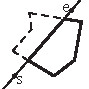
\includegraphics[width=\textwidth]{../code/Geometry/Polygon/PolygonCut}
\vspace{-6mm}
\end{minipage}
\begin{minted}[breaklines = true,
    breakanywhere = true,
    frame=lines,    
    fontfamily=tt,
    linenos=false,
    numberblanklines=true,
    numbersep=2pt,
    gobble=0,
    framerule=1pt,
    framesep=1mm,
    funcnamehighlighting=true,
    tabsize=1,
    obeytabs=false,
    mathescape=false
    samepage=false, %with this setting you can force the list to appear on the same page
    showspaces=false,
    showtabs =false,
    texcl=false]{C++}
/* Usage:
 *  vector<P> p = ...;
 *  p = polygonCut(p, P(0,0), P(1,0));
 * Status: tested but not extensively
 */
#include "Point.h"
#include "lineIntersection.h"

typedef Point<double> P;
vector<P> polygonCut(const vector<P>& poly, P s, P e) {
  vector<P> res;
  rep(i,0,sz(poly)) {
    P cur = poly[i], prev = i ? poly[i-1] : poly.back();
    bool side = s.cross(e, cur) < 0;
    if (side != (s.cross(e, prev) < 0))
      res.push_back(lineInter(s, e, cur, prev).second);
    if (side)
      res.push_back(cur);
  }
  return res;
}
\end{minted}

\subsection{Closest Pair}
Finds the closest pair of points.\\
Time: $O(n \log n)$
\begin{minted}[breaklines = true,
    breakanywhere = true,
    frame=lines,    
    fontfamily=tt,
    linenos=false,
    numberblanklines=true,
    numbersep=2pt,
    gobble=0,
    framerule=1pt,
    framesep=1mm,
    funcnamehighlighting=true,
    tabsize=1,
    obeytabs=false,
    mathescape=false
    samepage=false, %with this setting you can force the list to appear on the same page
    showspaces=false,
    showtabs =false,
    texcl=false]{C++}
#include "Point.h"

typedef Point<ll> P;
pair<P, P> closest(vector<P> v) {
  assert(sz(v) > 1);
  set<P> S;
  sort(all(v), [](P a, P b) { return a.y < b.y; });
  pair<ll, pair<P, P>> ret{LLONG_MAX, {P(), P()}};
  int j = 0;
  for (P p : v) {
    P d{1 + (ll)sqrt(ret.first), 0};
    while (v[j].y <= p.y - d.x) S.erase(v[j++]);
    auto lo = S.lower_bound(p - d), hi = S.upper_bound(p + d);
    for (; lo != hi; ++lo)
      ret = min(ret, {(*lo - p).dist2(), {*lo, p}});
    S.insert(p);
  }
  return ret.second;
}
\end{minted}

\subsection{Convex Hull}
\begin{minted}[
    breaklines = true,
    breakanywhere = true,
    frame=lines,    
    fontfamily=tt,
    linenos=false,
    numberblanklines=true,
    numbersep=2pt,
    gobble=0,
    framerule=1pt,
    framesep=1mm,
    funcnamehighlighting=true,
    tabsize=1,
    obeytabs=false,
    mathescape=false
    samepage=false, %with this setting you can force the list to appear on the same page
    showspaces=false,
    showtabs =false,
    texcl=false
]{C++}

typedef long long ll;
typedef pair <ll, ll> point;

#define x first
#define y second

inline ll area (point a, point b, point c) {
  return (b.x - a.x) * (c.y - a.y) - (b.y - a.y) * (c.x - a.x);
}

vector <point> convexHull (vector <point> p) {
  int n = p.size(), m = 0;
  if (n < 3) return p;
  vector <point> hull(n + n);
  sort(p.begin(), p.end());
  for (int i = 0; i < n; ++i) {
    while (m > 1 and area(hull[m - 2], hull[m - 1], p[i]) <= 0) --m;
    hull[m++] = p[i];
  }
  for (int i = n - 2, j = m + 1; i >= 0; --i) {
    while (m >= j and area(hull[m - 2], hull[m - 1], p[i]) <= 0) --m;
    hull[m++] = p[i];
  }
  hull.resize(m - 1); return hull;
}
\end{minted}

\subsection{Minimum Enclosing Circle}
\begin{minted}[
    breaklines = true,
    breakanywhere = true,
    frame=lines,    
    fontfamily=tt,
    linenos=false,
    numberblanklines=true,
    numbersep=2pt,
    gobble=0,
    framerule=1pt,
    framesep=1mm,
    funcnamehighlighting=true,
    tabsize=1,
    obeytabs=false,
    mathescape=false
    samepage=false, %with this setting you can force the list to appear on the same page
    showspaces=false,
    showtabs =false,
    texcl=false
]{C++}

// Expected runtime: O(n)
// Solves Gym 102299J


using namespace std;

typedef long double ld;
typedef pair <ld, ld> point;

#define x first
#define y second

point operator + (const point &a, const point &b) {
  return point(a.x + b.x, a.y + b.y);
}

point operator - (const point &a, const point &b) {
  return point(a.x - b.x, a.y - b.y);
}

point operator * (const point &a, const ld &b) {
  return point(a.x * b, a.y * b);
}

point operator / (const point &a, const ld &b) {
  return point(a.x / b, a.y / b);
}

const ld EPS = 1e-8;
const ld INF = 1e20;
const ld PI = acosl(-1);

inline ld dist (point a, point b) {
  return hypotl(a.x - b.x, a.y - b.y);
}

inline ld sqDist (point a, point b) {
  return (a.x - b.x) * (a.x - b.x) + (a.y - b.y) * (a.y - b.y);
}

inline ld dot (point a, point b) {
  return a.x * b.x + a.y * b.y;
}

inline ld cross (point a, point b) {
  return a.x * b.y - a.y * b.x;
}

inline ld cross (point a, point b, point c) {
  return cross(b - a, c - a);
}

inline point perp (point a) {
  return point(-a.y, a.x);
}

// circle through 3 points
pair <point, ld> getCircle (point a, point b, point c) {
  pair <point, ld> ret;
  ld den = (ld) 2 * cross(a, b, c);
  ret.x.x = ((c.y - a.y) * (dot(b, b) - dot(a, a)) - (b.y - a.y) * (dot(c, c) - dot(a, a))) / den;
  ret.x.y = ((b.x - a.x) * (dot(c, c) - dot(a, a)) - (c.x - a.x) * (dot(b, b) - dot(a, a))) / den;
  ret.y = dist(ret.x, a);
  return ret;
}

pair <point, ld> minCircleAux (vector <point> &s, point a, point b, int n) {
  ld lo = -INF, hi = INF;
  for (int i = 0; i < n; ++i) {
    auto si = cross(b - a, s[i] - a);
    if (fabs(si) < EPS) continue;
    point m = getCircle(a, b, s[i]).x;
    auto cr = cross(b - a, m - a);
    si < 0 ? hi = min(hi, cr) : lo = max(lo, cr);
  }
  ld v = 0 < lo ? lo : hi < 0 ? hi : 0;
  point c = (a + b) * 0.5 + perp(b - a) * v / sqDist(a, b);
  return {c, sqDist(a, c)};
}

pair <point, ld> minCircle (vector <point> &s, point a, int n) {
  random_shuffle(s.begin(), s.begin() + n);
  point b = s[0], c = (a + b) * 0.5;
  ld r = sqDist(a, c);
  for (int i = 1; i < n; ++i) {
    if (sqDist(s[i], c) > r * (1 + EPS)) {
      tie(c, r) = n == s.size() ? minCircle(s, s[i], i) : minCircleAux(s, a, s[i], i);
    }
  }
  return {c, r};
}

pair <point, ld> minCircle (vector <point> s) {
  assert(!s.empty());
  if (s.size() == 1) return {s[0], 0};
  return minCircle(s, s[0], s.size());
}

int n; vector <point> p;

int main() {
  cin >> n;
  while (n--) {
    double x, y;
    scanf("%lf %lf", &x, &y);
    p.emplace_back(x, y);
  }
  pair <point, ld> circ = minCircle(p);
  printf("%0.12f %0.12f %0.12f\n", (double) circ.x.x, (double) circ.x.y, (double) (0.5 * circ.y));
  return 0;
}
\end{minted}

\subsection{Point In Polygon}
\begin{minted}[
    breaklines = true,
    breakanywhere = true,
    frame=lines,    
    fontfamily=tt,
    linenos=false,
    numberblanklines=true,
    numbersep=2pt,
    gobble=0,
    framerule=1pt,
    framesep=1mm,
    funcnamehighlighting=true,
    tabsize=1,
    obeytabs=false,
    mathescape=false
    samepage=false, %with this setting you can force the list to appear on the same page
    showspaces=false,
    showtabs =false,
    texcl=false
]{C++}

// Test if a point is inside a convex polygon in O(lg n) time
// Solves SPOJ INOROUT
typedef long long ll;
typedef pair <ll, ll> point;

#define x first
#define y second

struct segment {
  point P1, P2;

  segment () {}
  segment (point P1, point P2) : P1(P1), P2(P2) {}
};

inline ll ccw (point A, point B, point C) {
  return (B.x - A.x) * (C.y - A.y) - (C.x - A.x) * (B.y - A.y);
}

inline bool pointOnSegment (segment S, point P) {
  ll x = P.x, y = P.y, x1 = S.P1.x, y1 = S.P1.y, x2 = S.P2.x, y2 = S.P2.y;
  ll a = x - x1, b = y - y1, c = x2 - x1, d = y2 - y1, dot = a * c + b * d, len = c * c + d * d;
  if (x1 == x2 and y1 == y2) return x1 == x and y1 == y;
  if (dot < 0 or dot > len) return 0;
  return x1 * len + dot * c == x * len and y1 * len + dot * d == y * len;
}

const int M = 17;
const int N = 10010;

struct polygon {
  int n; // n > 1
  point p[N]; // clockwise order

  polygon () {}
  polygon (int _n, point *T) {
    n = _n;
    for (int i = 0; i < n; ++i) p[i] = T[i];
  }

  bool contains (point P, bool strictlyInside) {
    int lo = 1, hi = n - 1;
    while (lo < hi){
      int mid = lo + hi >> 1;
      if (ccw(p[0], P, p[mid]) > 0) lo = mid + 1;
      else hi = mid;
    }
    if (ccw(p[0], P, p[lo]) > 0) lo = 1;
    if (!strictlyInside and pointOnSegment(segment(p[0], p[n - 1]), P)) return 1;
    if (!strictlyInside and pointOnSegment(segment(p[lo], p[lo - 1]), P)) return 1;
    if (lo == 1 or ccw(p[0], P, p[n - 1]) == 0) return 0;
    return ccw(p[lo], P, p[lo - 1]) < 0;
  }
};
\end{minted}

\subsection{near\_pair}
\begin{minted}[
    breaklines = true,
    breakanywhere = true,
    frame=lines,    
    fontfamily=tt,
    linenos=false,
    numberblanklines=true,
    numbersep=2pt,
    gobble=0,
    framerule=1pt,
    framesep=1mm,
    funcnamehighlighting=true,
    tabsize=1,
    obeytabs=false,
    mathescape=false
    samepage=false, %with this setting you can force the list to appear on the same page
    showspaces=false,
    showtabs =false,
    texcl=false
]{C++}

struct pt {
  int x, y, id;
};

struct cmp_x {
  bool operator()(const pt & a, const pt & b) const {
    return a.x < b.x || (a.x == b.x && a.y < b.y);
  }
};

struct cmp_y {
  bool operator()(const pt & a, const pt & b) const {
    return a.y < b.y;
  }
};

int n;
vector<pt> a;
double mindist;
pair<int, int> best_pair;

void upd_ans(const pt & a, const pt & b) {
  double dist = sqrt((a.x - b.x)*(a.x - b.x) + (a.y - b.y)*(a.y - b.y));
  if (dist < mindist) {
    mindist = dist;
    best_pair = {a.id, b.id};
  }
}
vector<pt> t;

void rec(int l, int r) {
  if (r - l <= 3) {
    for (int i = l; i < r; ++i) {
      for (int j = i + 1; j < r; ++j) {
        upd_ans(a[i], a[j]);
      }
    }
    sort(a.begin() + l, a.begin() + r, cmp_y());
    return;
  }

  int m = (l + r) >> 1;
  int midx = a[m].x;
  rec(l, m);
  rec(m, r);

  merge(a.begin() + l, a.begin() + m, a.begin() + m, a.begin() + r, t.begin(), cmp_y());
  copy(t.begin(), t.begin() + r - l, a.begin() + l);

  int tsz = 0;
  for (int i = l; i < r; ++i) {
    if (abs(a[i].x - midx) < mindist) {
      for (int j = tsz - 1; j >= 0 && a[i].y - t[j].y < mindist; --j)
        upd_ans(a[i], t[j]);
      t[tsz++] = a[i];
    }
  }
}

void solve(int n)
{
  t.resize(n);
  sort(a.begin(), a.end(), cmp_x());
  mindist = 1E20;
  rec(0, n);
}
\end{minted}

\subsection{sweep}
\begin{minted}[
    breaklines = true,
    breakanywhere = true,
    frame=lines,    
    fontfamily=tt,
    linenos=false,
    numberblanklines=true,
    numbersep=2pt,
    gobble=0,
    framerule=1pt,
    framesep=1mm,
    funcnamehighlighting=true,
    tabsize=1,
    obeytabs=false,
    mathescape=false
    samepage=false, %with this setting you can force the list to appear on the same page
    showspaces=false,
    showtabs =false,
    texcl=false
]{C++}

const double EPS = 1E-9;

struct pt {
  double x, y;
};

struct seg {
  pt p, q;
  int id;

  double get_y(double x) const {
    if (abs(p.x - q.x) < EPS)
      return p.y;
    return p.y + (q.y - p.y) * (x - p.x) / (q.x - p.x);
  }
};

bool intersect1d(double l1, double r1, double l2, double r2) {
  if (l1 > r1)
    swap(l1, r1);
  if (l2 > r2)
    swap(l2, r2);
  return max(l1, l2) <= min(r1, r2) + EPS;
}

int vec(const pt& a, const pt& b, const pt& c) {
  double s = (b.x - a.x) * (c.y - a.y) - (b.y - a.y) * (c.x - a.x);
  return abs(s) < EPS ? 0 : s > 0 ? +1 : -1;
}

bool intersect(const seg& a, const seg& b)
{
  return intersect1d(a.p.x, a.q.x, b.p.x, b.q.x) &&
    intersect1d(a.p.y, a.q.y, b.p.y, b.q.y) &&
    vec(a.p, a.q, b.p) * vec(a.p, a.q, b.q) <= 0 &&
    vec(b.p, b.q, a.p) * vec(b.p, b.q, a.q) <= 0;
}

bool operator<(const seg& a, const seg& b)
{
  double x = max(min(a.p.x, a.q.x), min(b.p.x, b.q.x));
  return a.get_y(x) < b.get_y(x) - EPS;
}

struct event {
  double x;
  int tp, id;

  event() {}
  event(double x, int tp, int id) : x(x), tp(tp), id(id) {}

  bool operator<(const event& e) const {
    if (abs(x - e.x) > EPS)
      return x < e.x;
    return tp > e.tp;
  }
};

set<seg> s;
vector<set<seg>::iterator> where;

set<seg>::iterator prev(set<seg>::iterator it) {
  return it == s.begin() ? s.end() : --it;
}

set<seg>::iterator next(set<seg>::iterator it) {
  return ++it;
}

pair<int, int> solve(const vector<seg>& a) {
  int n = (int)a.size();
  vector<event> e;
  for (int i = 0; i < n; ++i) {
    e.push_back(event(min(a[i].p.x, a[i].q.x), +1, i));
    e.push_back(event(max(a[i].p.x, a[i].q.x), -1, i));
  }
  sort(e.begin(), e.end());

  s.clear();
  where.resize(a.size());
  for (size_t i = 0; i < e.size(); ++i) {
    int id = e[i].id;
    if (e[i].tp == +1) {
      set<seg>::iterator nxt = s.lower_bound(a[id]), prv = prev(nxt);
      if (nxt != s.end() && intersect(*nxt, a[id]))
        return make_pair(nxt->id, id);
      if (prv != s.end() && intersect(*prv, a[id]))
        return make_pair(prv->id, id);
      where[id] = s.insert(nxt, a[id]);
    } else {
      set<seg>::iterator nxt = next(where[id]), prv = prev(where[id]);
      if (nxt != s.end() && prv != s.end() && intersect(*nxt, *prv))
        return make_pair(prv->id, nxt->id);
      s.erase(where[id]);
    }
  }

  return make_pair(-1, -1);
}
\end{minted}

\section{Graph}
\subsection{2Sat}
\begin{minted}[
    breaklines = true,
    breakanywhere = true,
    frame=lines,    
    fontfamily=tt,
    linenos=false,
    numberblanklines=true,
    numbersep=2pt,
    gobble=0,
    framerule=1pt,
    framesep=1mm,
    funcnamehighlighting=true,
    tabsize=1,
    obeytabs=false,
    mathescape=false
    samepage=false, %with this setting you can force the list to appear on the same page
    showspaces=false,
    showtabs =false,
    texcl=false
]{C++}

namespace sat{
  const int MAX = 200010;
  bool vis[MAX];
  vector <int> ed[MAX], rev[MAX];
  int n, m, ptr, dfs_t[MAX], ord[MAX], par[MAX];

  inline int inv(int x){
    return ((x) <= n ? (x + n) : (x - n));
  }

  void init(int vars){
    n = vars, m = vars << 1;
    for (int i = 1; i <= m; i++){
      ed[i].clear();
      rev[i].clear();
    }
  }

  inline void add(int a, int b){
    ed[a].push_back(b);
    rev[b].push_back(a);
  }


  inline void OR(int a, int b){
    add(inv(a), b);
    add(inv(b), a);
  }

  inline void AND(int a, int b){
    add(a, b);
    add(b, a);
  }

  void XOR(int a,int b){
    add(inv(b), a);
    add(a, inv(b));
    add(inv(a), b);
    add(b, inv(a));
  }

  inline void XNOR(int a, int b){
    add(a,b);
    add(b,a);
    add(inv(a), inv(b));
    add(inv(b), inv(a));
  }

  inline void force_true(int x){
    add(inv(x), x);
  }

  inline void topsort(int s){
    vis[s] = true;
    for(int x : rev[s]) if(!vis[x]) topsort(x);
    dfs_t[s] = ++ptr;
  }

  inline void dfs(int s, int p){
    par[s] = p;
    vis[s] = true;
    for(int x : ed[s]) if (!vis[x]) dfs(x, p);
  }

  void build(){
    CLR(vis);
    ptr = 0;
    for(int i=m;i>=1;i--) {
      if (!vis[i]) topsort(i);
      ord[dfs_t[i]] = i;
    }
    CLR(vis);
    for (int i = m; i >= 1; i--){
      int x = ord[i];
      if (!vis[x]) dfs(x, x);
    }
  }

  bool satisfy(vector <int>& res){
    build();
    CLR(vis);

    for (int i = 1; i <= m; i++){
      int x = ord[i];
      if (par[x] == par[inv(x)]) return false;
      if (!vis[par[x]]){
        vis[par[x]] = true;
        vis[par[inv(x)]] = false;
      }
    }
    res.clear();
    for (int i = 1; i <= n; i++){
      if (vis[par[i]]) res.push_back(i);
    }
    return true;
  }
}
\end{minted}

\subsection{Centroid\_decomp}
\begin{minted}[
    breaklines = true,
    breakanywhere = true,
    frame=lines,    
    fontfamily=tt,
    linenos=false,
    numberblanklines=true,
    numbersep=2pt,
    gobble=0,
    framerule=1pt,
    framesep=1mm,
    funcnamehighlighting=true,
    tabsize=1,
    obeytabs=false,
    mathescape=false
    samepage=false, %with this setting you can force the list to appear on the same page
    showspaces=false,
    showtabs =false,
    texcl=false
]{C++}

vector <int> ed[MAX];
bool isCentroid[MAX];
int sub[MAX], cpar[MAX], clevel[MAX];
int dis[20][MAX];

void calcSubTree(int s,int p) {
  sub[s] = 1;
  for(int x : ed[s]) {
    if(x == p or isCentroid[x]) continue;
    calcSubTree(x,s);
    sub[s] += sub[x];
  }
}

int nn;

int getCentroid(int s,int p) {
  for(int x : ed[s]) {
    if(!isCentroid[x] && x!=p && sub[x]>(nn/2)) return getCentroid(x,s);
  }
  return s;
}

void setDis(int s, int from, int p, int lev) {
  dis[from][s] = lev;
  for(int x : ed[s]) {
    if(x == p or isCentroid[x] )  continue;
    setDis(x, from, s, lev+1);
  }
}

void decompose(int s,int p,int lev) {
  calcSubTree(s,p);
  nn = sub[s];
  int c = getCentroid(s,p);
  setDis(c,lev,p,0);

  isCentroid[c] = true;
  cpar[c] = p;
  clevel[c] = lev;

  for(int x : ed[c]) {
    if(!isCentroid[x]) decompose(x,c,lev+1);
  }
}

int ans[MAX];

inline void update(int v) {
  int u = v;
  while(u!=-1) {
    ans[u] = min(ans[u], dis[clevel[u]][v]);
    u = cpar[u];
  }
}

inline int query(int v) {
  int ret = INF;
  int u = v;
  while(u != -1) {
    ret = min(ret, dis[clevel[u]][v]+ans[u]);
    u = cpar[u];
  }
  return ret;
}
int main() {
  decompose(1,-1,0);
  for(int i=1; i<=n; i++) ans[i] = INF;
  update(v);
  query(v));
  return 0;
}
\end{minted}

\subsection{articulation\_point}
\begin{minted}[
    breaklines = true,
    breakanywhere = true,
    frame=lines,    
    fontfamily=tt,
    linenos=false,
    numberblanklines=true,
    numbersep=2pt,
    gobble=0,
    framerule=1pt,
    framesep=1mm,
    funcnamehighlighting=true,
    tabsize=1,
    obeytabs=false,
    mathescape=false
    samepage=false, %with this setting you can force the list to appear on the same page
    showspaces=false,
    showtabs =false,
    texcl=false
]{C++}

using namespace std;

const int N = 1e5 + 10;
vector<int> g[N];
int vis[N], low[N], cut[N], now = 0, n, m;

void dfs(int u, int p) {
  low[u] = vis[u] = ++now; int ch = 0;
  for(int v : g[u]){
    if(v ^ p) {
      if(vis[v]) low[u] = min(low[u], vis[v]);
      else {
        ch++; dfs(v, u);
        low[u] = min(low[u], low[v]);
        if(p + 1 && low[v] >= vis[u]) cut[u] = 1;
        if(low[v] > vis[u]) {
          printf("Bridge %d -- %d\n", u, v);
        }
      }
    }
  } if(p == -1 && ch > 1) cut[u] = 1;
}

void ArticulationPointAndBridge() {
  now = 0;
  for(int i = 0; i < n; i++) {
    if(!vis[i]) dfs(i, -1);
  }
}
\end{minted}

\subsection{bcc}
\begin{minted}[
    breaklines = true,
    breakanywhere = true,
    frame=lines,    
    fontfamily=tt,
    linenos=false,
    numberblanklines=true,
    numbersep=2pt,
    gobble=0,
    framerule=1pt,
    framesep=1mm,
    funcnamehighlighting=true,
    tabsize=1,
    obeytabs=false,
    mathescape=false
    samepage=false, %with this setting you can force the list to appear on the same page
    showspaces=false,
    showtabs =false,
    texcl=false
]{C++}

// clear ed[] every test case
// tot -> total number of components
// bcc[i] contains the nodes of the i'th component
// any self loop or multiple edge?

const int MAX = ?;
vector <int> ed[MAX];
bool cut[MAX];
int tot, Time, low[MAX], st[MAX];
vector <int> bcc[MAX];
stack <int> S;

void popBCC(int s,int x) {
  cut[s] = 1;
  bcc[++tot].pb(s);
  while(bcc[tot].back() ^ x) {
    bcc[tot].pb(S.top());
    S.pop();
  }
}

void dfs(int s, int p = -1) {
  S.push(s);
  int ch = 0;
  st[s] = low[s] = ++Time;
  for(int x : ed[s]) {
    if(!st[x]) {
      ch++;
      dfs(x,s);
      low[s] = min(low[s],low[x]);
      if(p != -1 and low[x] >= st[s]) popBCC(s,x);
      else if(p == -1) if(ch > 1) popBCC(s,x);
    }
    else if(p != x) low[s] = min(low[s],st[x]);
  }
  if(p == -1 && ch > 1) cut[s] = 1;
}

void processBCC(int n) {
  for(int i=1;i<=n;i++) bcc[i].clear();
  CLR(st); CLR(cut);
  Time = tot = 0;
  for(int i=1; i<=n; i++) {
    if(!st[i]) {
      dfs(i,-1);
      if(!S.empty()) ++tot;
      while(!S.empty()) {
        bcc[tot].push_back(S.top());
        S.pop();
      }
    }
  }
}
\end{minted}

\subsection{bridge\_tree}
\begin{minted}[
    breaklines = true,
    breakanywhere = true,
    frame=lines,    
    fontfamily=tt,
    linenos=false,
    numberblanklines=true,
    numbersep=2pt,
    gobble=0,
    framerule=1pt,
    framesep=1mm,
    funcnamehighlighting=true,
    tabsize=1,
    obeytabs=false,
    mathescape=false
    samepage=false, %with this setting you can force the list to appear on the same page
    showspaces=false,
    showtabs =false,
    texcl=false
]{C++}

const int MAXN = ?;
const int MAXE = ?;

struct edges {
  int u,v;
} ara[MAXE];

vector <int> ed[MAXN];
vector <int> isBridge[MAXN];
vector <int> brTree[MAXN];

bool vis[MAXN];
int st[MAXN], low[MAXN], Time = 0;
int cnum;
int comp[MAXN];

void findBridge(int s,int par) {
  int i,x,child = 0,j;
  vis[s] = 1;
  Time++;
  st[s] = low[s] = Time;
  for(i=0; i<ed[s].size(); i++) {
    x = ed[s][i];
    if(!vis[x]) {
      child++;
      findBridge(x,s);
      low[s] = min(low[s],low[x]);
      if(low[x] > st[s]) {
        isBridge[s][i] = 1;
        j = lower_bound(ed[x].begin(),ed[x].end(),s)-ed[x].begin();
        isBridge[x][j] = 1;
      }
    }
    else if(par!=x)
      low[s] = min(low[s],st[x]);
  }
}

void dfs(int s) {
  int i,x;
  vis[s] = 1;
  comp[s] = cnum;
  for(i=0; i<ed[s].size(); i++) {
    if(!isBridge[s][i]) {
      x = ed[s][i];
      if(!vis[x]) dfs(x);
    }
  }
}

void processBridge(int n,int m) {
  CLR(vis);
  Time = 0;
  for(int i=1; i<=n; i++) if(!vis[i]) findBridge(i,-1);

  cnum = 0;
  CLR(vis);
  for(int i=1; i<=n; i++) {
    if(!vis[i]) {
      cnum++;
      dfs(i);
    }
  }

  n = cnum;

  for(int i=1; i<=m; i++) {
    if(comp[ara[i].u] != comp[ara[i].v]) {
      brTree[comp[ara[i].u]].pb(comp[ara[i].v]);
      brTree[comp[ara[i].v]].pb(comp[ara[i].u]);
    }
  }
}



int main() {
  int n,m,u,v;
  scanf("%d %d",&n,&m);
  for(int i=1; i<=m; i++) {
    sii(u,v);

    ed[u].pb(v);
    ed[v].pb(u);

    isBridge[u].pb(0);
    isBridge[v].pb(0);

    ara[i].u = u;
    ara[i].v = v;
  }
  for(int i=1; i<=n; i++) sort(all(ed[i]));
  processBridge(n,m);
  return 0;
}
\end{minted}

\subsection{dinic}
\begin{minted}[
    breaklines = true,
    breakanywhere = true,
    frame=lines,    
    fontfamily=tt,
    linenos=false,
    numberblanklines=true,
    numbersep=2pt,
    gobble=0,
    framerule=1pt,
    framesep=1mm,
    funcnamehighlighting=true,
    tabsize=1,
    obeytabs=false,
    mathescape=false
    samepage=false, %with this setting you can force the list to appear on the same page
    showspaces=false,
    showtabs =false,
    texcl=false
]{C++}

namespace dinic {
  using T = int;
  const T INF = 0x3f3f3f3f;
  const int MAXN = 5010;

  int n, src, snk, work[MAXN];
  T dist[MAXN];

  struct Edge{
    int to, rev_pos;
    T c, f;
  };
  vector <Edge> ed[MAXN];

  void init(int _n, int _src, int _snk) {
    n = _n, src = _src, snk = _snk;
    for(int i=1;i<=n;i++) ed[i].clear();
  }

  inline void addEdge(int u, int v, T c, T rc = 0) {
    Edge a = {v, (int)ed[v].size(), c, 0};
    Edge b = {u, (int)ed[u].size(), rc, 0};
    ed[u].push_back(a);
    ed[v].push_back(b);
  }

  bool dinic_bfs() {
    SET(dist);
    dist[src] = 0;
    queue <int> q;
    q.push(src);
    while(!q.empty()){
      int u = q.front(); q.pop();
      for(Edge &e : ed[u]){
        if(dist[e.to] == -1 and e.f < e.c) {
          dist[e.to] = dist[u] + 1;
          q.push(e.to);
        }
      }
    }
    return (dist[snk]>=0);
  }

  T dinic_dfs(int u, T fl){
    if (u == snk) return fl;
    for (; work[u] < (int)ed[u].size(); work[u]++) {
      Edge &e = ed[u][work[u]];
      if (e.c <= e.f) continue;
      int v = e.to;
      if (dist[v] == dist[u] + 1){
        T df = dinic_dfs(v, min(fl, e.c - e.f));
        if (df > 0){
          e.f += df;
          ed[v][e.rev_pos].f -= df;
          return df;
        }
      }
    }
    return 0;
  }
  T solve() {
    T ret = 0;
    while (dinic_bfs()) {
      CLR(work);
      while (T delta = dinic_dfs(src, INF)) ret += delta;
    }
    return ret;
  }
}


int main() {
  int n, m, u, v, c;
  cin >> n >> m;
  dinic::init(n, 1, n);
  while(m--) {
    cin >> u >> v >> c;
    dinic::addEdge(u, v, c, c);
  }
  cout << dinic::solve() << '\n';
  return 0;
}
\end{minted}

\subsection{dsu\_on\_tree}
\begin{minted}[
    breaklines = true,
    breakanywhere = true,
    frame=lines,    
    fontfamily=tt,
    linenos=false,
    numberblanklines=true,
    numbersep=2pt,
    gobble=0,
    framerule=1pt,
    framesep=1mm,
    funcnamehighlighting=true,
    tabsize=1,
    obeytabs=false,
    mathescape=false
    samepage=false, %with this setting you can force the list to appear on the same page
    showspaces=false,
    showtabs =false,
    texcl=false
]{C++}

void calcSubSize(int s,int p) {
  sub[s] = 1;
  for(int x : G[s]) {
    if(x==p) continue;
    calcSubSize(x,s);
    sub[s] += sub[x];
  }
}
void add(int s,int p,int v,int bigchild = -1) {
  freq[color[s]] += v;
  for(int x : G[s]) {
    if(x==p || x==bigchild) continue;
    add(x,s,v);
  }
}
void dfs(int s,int p,bool keep) {
  int bigChild = -1;
  for(int x : G[s]) {
    if(x==p) continue;
    if(bigChild==-1 || sub[bigChild] < sub[x] ) bigChild = x;
  }
  for(int x : G[s]) {
    if(x==p || x==bigChild) continue;
    dfs(x,s,0);
  }
  if(bigChild!=-1) dfs(bigChild,s,1);
  add(s,p,1,bigChild);
  if(keep==0)
    add(s,p,-1);
}
\end{minted}

\subsection{euler\_path}
\begin{minted}[
    breaklines = true,
    breakanywhere = true,
    frame=lines,    
    fontfamily=tt,
    linenos=false,
    numberblanklines=true,
    numbersep=2pt,
    gobble=0,
    framerule=1pt,
    framesep=1mm,
    funcnamehighlighting=true,
    tabsize=1,
    obeytabs=false,
    mathescape=false
    samepage=false, %with this setting you can force the list to appear on the same page
    showspaces=false,
    showtabs =false,
    texcl=false
]{C++}

vector <int> ed[MAX+5], sltn;

int inDeg[MAX+5], outDeg[MAX+5];
bool vis[MAX+5];

void dfs(int nd) {
  vis[nd] = true;
  while(ed[nd].size()) {
    int v = ed[nd].back();
    ed[nd].pop_back();
    dfs(v);
  }
  sltn.pb(nd);
}

int findEuler (int n) {
  int src , snk , ret = 1;
  bool found_src = false, found_snk = false;
  CLR(inDeg); CLR(outDeg);
  for(int u = 1; u <= n; u++) {
    for(int i = 0; i<ed[u].size(); i++) {
      int v = ed[u][i];
      outDeg[u]++;
      inDeg[v]++;
    }
  }
  int diff;
  for(int i = 1; i<=n; i++) {
    diff = outDeg[i] - inDeg[i];
    if(diff == 1) {
      if(found_src) return 0;
      found_src = true;
      src = i;
    }
    else if (diff == -1) {
      if(found_snk) return 0;
      found_snk = true;
      snk = i;
    }
    else if(diff != 0) return 0;
  }
  if(!found_src) {
    ret = 2;
    for(int i = 1 ; i <= n ; i++) {
      if( outDeg[i] ) {
        found_src = true;
        src = i;
        break;
      }
    }
  }
  if(!found_src) return ret;
  CLR(vis);
  sltn.clear();
  dfs(src);
  for(int i = 1; i<=n; i++) {
    if(outDeg[i] && !vis[i]) return 0;
  }
  for(int i = (int)sltn.size()-1; i>=0; i--) printf("%d ",sltn[i]);
  puts("");

  return ret;
}
\end{minted}

\subsection{hld}
\begin{minted}[
    breaklines = true,
    breakanywhere = true,
    frame=lines,    
    fontfamily=tt,
    linenos=false,
    numberblanklines=true,
    numbersep=2pt,
    gobble=0,
    framerule=1pt,
    framesep=1mm,
    funcnamehighlighting=true,
    tabsize=1,
    obeytabs=false,
    mathescape=false
    samepage=false, %with this setting you can force the list to appear on the same page
    showspaces=false,
    showtabs =false,
    texcl=false
]{C++}

const int N = 3e4 + 5;
vector<int> G[N];
int sz[N], H[N], P[N];

void dfs(int cur, int h)
{
    sz[cur] = 1;
    H[cur] = h;
    for(int& to : G[cur]) {
        G[to].erase(find(G[to].begin(), G[to].end(), cur));
        P[to] = cur;
        dfs(to, h + 1);
        sz[cur] += sz[to];
        if(sz[to] > sz[G[cur][0]]) swap(G[cur][0], to);
    }
}

int base[N], pos[N], head[N];
int ptr = 0;

void hld(int cur)
{
    pos[cur] = ++ptr;
    base[ptr] = cur;
    for(int to : G[cur]) {
        head[to] = (to == G[cur][0] ? head[cur] : to);
        hld(to);
    }
}

segtree ST;

int query(int u, int v)
{
    int ret = 0;
    while(head[u] != head[v]) {
        if(H[head[u]] > H[head[v]]) swap(u, v);
        ret += ST.query(pos[head[v]], pos[v]);
        v = P[head[v]];
    }
    if(H[u] > H[v]) swap(u, v);
    ret += ST.query(pos[u], pos[v]);
    return ret;
}

void update(int u, int val) {
    ST.update(pos[u], val);
}

void build(int n, int root)
{
    ptr = 0;
    dfs(root, 0);
    head[root] = root;
    hld(root);
    ST = segtree(n);
}

/*
 * clear graph
 * call build
 * Prob : sum of values from u to v
 */
\end{minted}

\subsection{hopcroft\_karp}
\begin{minted}[
    breaklines = true,
    breakanywhere = true,
    frame=lines,    
    fontfamily=tt,
    linenos=false,
    numberblanklines=true,
    numbersep=2pt,
    gobble=0,
    framerule=1pt,
    framesep=1mm,
    funcnamehighlighting=true,
    tabsize=1,
    obeytabs=false,
    mathescape=false
    samepage=false, %with this setting you can force the list to appear on the same page
    showspaces=false,
    showtabs =false,
    texcl=false
]{C++}

struct HopcroftKarp {
  const int N, M;
  std::vector<std::vector<int>> adj_left;
  std::vector<int> matchL, matchR;

  HopcroftKarp(int N, int M, const std::vector<std::pair<int, int>>& edge)
      : N(N), M(M), matchL(N, -1), matchR(M, -1), adj_left(N) {
    for (auto [l, r] : edge)
      adj_left[l].push_back(r);
  }

  int maxmatching() {
    int sz = 0;
    for (bool updated = true; updated;) {
      updated = false;
      static std::vector<int> root(N), prev(N), qq(N);
      static int qi, qj;
      // std::queue<int> q;
      qi = qj = 0;
      std::fill(root.begin(), root.end(), -1),
      std::fill(prev.begin(), prev.end(), -1);
      for (int i = 0; i < N; i++)
        if (matchL[i] == -1)
          qq[qj++] = i, root[i] = i, prev[i] = i;
      // q.push(i), root[i] = i;
      while (qi < qj) {
        int u = qq[qi++];
        // int u = q.front(); q.pop();
        if (matchL[root[u]] != -1) continue;
        for (int v : adj_left[u]) {
          if (matchR[v] == -1) {
            while (v != -1)
              matchR[v] = u, std::swap(matchL[u], v), u = prev[u];
            updated = true, sz++;
            break;
          }
          if (prev[matchR[v]] == -1)
            v = matchR[v], prev[v] = u, root[v] = root[u], qq[qj++] = v;
          // v = matchR[v], prev[v] = u, root[v] = root[u], q.push(v);
        }
      }
    }
    return sz;
  }
};
\end{minted}

\subsection{hungarian}
\begin{minted}[
    breaklines = true,
    breakanywhere = true,
    frame=lines,    
    fontfamily=tt,
    linenos=false,
    numberblanklines=true,
    numbersep=2pt,
    gobble=0,
    framerule=1pt,
    framesep=1mm,
    funcnamehighlighting=true,
    tabsize=1,
    obeytabs=false,
    mathescape=false
    samepage=false, %with this setting you can force the list to appear on the same page
    showspaces=false,
    showtabs =false,
    texcl=false
]{C++}

// Given N×N matrix A[i][j]. Calculate a permutation p[i]​ that minimize ∑A[i][p[i]]​.
template <typename T>
pair <T, vector <int>> Hungarian (int n, int m, T c[N][N]) {
  vector <T> v(m), dist(m);
  vector <int> L(n, -1), R(m, -1);
  vector <int> index(m), prev(m);
  auto residue = [&] (int i, int j) {return c[i][j] - v[j];};

  iota(index.begin(), index.end(), 0);
  for (int f = 0; f < n; ++f) {
    for (int j = 0; j < m; ++j) {
      dist[j] = residue(f, j), prev[j] = f;
    }
    T w; int i, j, l, s = 0, t = 0;
    while (true) {
      if (s == t) {
        l = s, w = dist[index[t++]];
        for (int k = t; k < m; ++k) {
          j = index[k]; T h = dist[j];
          if (h <= w) {
            if (h < w) t = s, w = h;
            index[k] = index[t], index[t++] = j;
          }
        }
        for (int k = s; k < t; ++k) {
          j = index[k];
          if (R[j] < 0) goto augment;
        }
      }
      int q = index[s++], i = R[q];
      for (int k = t; k < m; ++k) {
        j = index[k];
        T h = residue(i, j) - residue(i, q) + w;
        if (h < dist[j]) {
          dist[j] = h, prev[j] = i;
          if (h == w) {
            if (R[j] < 0) goto augment;
            index[k] = index[t], index[t++] = j;
          }
        }
      }
    }
  augment:
    for (int k = 0; k < l; ++k) v[index[k]] += dist[index[k]] - w;
    do {
      R[j] = i = prev[j], swap(j, L[i]);
    } while (i ^ f);
  }
  T ret = 0;
  for (int i = 0; i < n; ++i) ret += c[i][L[i]];
  return {ret, L};
}
\end{minted}

\subsection{kuhn}
\begin{minted}[
    breaklines = true,
    breakanywhere = true,
    frame=lines,    
    fontfamily=tt,
    linenos=false,
    numberblanklines=true,
    numbersep=2pt,
    gobble=0,
    framerule=1pt,
    framesep=1mm,
    funcnamehighlighting=true,
    tabsize=1,
    obeytabs=false,
    mathescape=false
    samepage=false, %with this setting you can force the list to appear on the same page
    showspaces=false,
    showtabs =false,
    texcl=false
]{C++}

namespace bpm{
  const int L = 105;
  const int R = 105;

  vector <int> G[L];
  int matchR[R], matchL[L], vis[L], it;

  void init(int n) {
    SET(matchL), SET(matchR), CLR(vis);
    it = 1;
    for(int i=1;i<=n;i++) G[i].clear();
  }

  inline void addEdge(int u,int v) { G[u].pb(v); }

  bool dfs(int s) {
    vis[s] = it;
    for(auto x : G[s]) {
      if( matchR[x] == -1 or (vis[matchR[x]] != it and dfs(matchR[x])) ) {
        matchL[s] = x; matchR[x] = s;
        return true;
      }
    }
    return false;
  }

  int solve() {
    int cnt = 0;
    for(int i=1;i<=n;i++) {
      if(dfs(i)) cnt++, it++;
    }
    return cnt;
  }
}
\end{minted}

\subsection{lca}
\begin{minted}[
    breaklines = true,
    breakanywhere = true,
    frame=lines,    
    fontfamily=tt,
    linenos=false,
    numberblanklines=true,
    numbersep=2pt,
    gobble=0,
    framerule=1pt,
    framesep=1mm,
    funcnamehighlighting=true,
    tabsize=1,
    obeytabs=false,
    mathescape=false
    samepage=false, %with this setting you can force the list to appear on the same page
    showspaces=false,
    showtabs =false,
    texcl=false
]{C++}

// Don't forget to clear ed after test case ends(vt, cost are cleared inside)

using namespace std;
const int MAX = 100010;

int LG;
int dep[MAX], par[MAX][21];
vector <int> ed[MAX];

void dfs(int s, int p, int d) {
  dep[s] = d, par[s][0] = p;
  for(int x : ed[s]) {
    if(x == p) continue;
    dfs(x, s, d+1);
  }
}

void preprocess(int root, int n) {
  LG = __lg(n);
  memset(par, -1, sizeof(par));
  dfs(root, -1, 0);

  for(int j=1;j<=LG;j++) {
    for(int i=1;i<=n;i++) {
      if(par[i][j-1] != -1) par[i][j] = par[par[i][j-1]][j-1];
    }
  }
}


int getLCA(int u, int v) {
  if(dep[u] < dep[v]) swap(u, v);
  for(int i=LG;i>=0;i--) {
    if(dep[u] - (1<<i) >= dep[v]) u = par[u][i];
  }
  if(u == v) return u;
  for(int i=LG;i>=0;i--) {
    if (par[u][i] != -1 and par[u][i] - par[v][i]) {
      u = par[u][i], v = par[v][i];
    }
  }
  return par[u][0];
}
\end{minted}

\subsection{manhattan\_MST}
\begin{minted}[
    breaklines = true,
    breakanywhere = true,
    frame=lines,    
    fontfamily=tt,
    linenos=false,
    numberblanklines=true,
    numbersep=2pt,
    gobble=0,
    framerule=1pt,
    framesep=1mm,
    funcnamehighlighting=true,
    tabsize=1,
    obeytabs=false,
    mathescape=false
    samepage=false, %with this setting you can force the list to appear on the same page
    showspaces=false,
    showtabs =false,
    texcl=false
]{C++}

using namespace std;
using ll = long long;
struct UnionFind {
    vector<int> UF;
    int cnt;
    UnionFind(int N) : UF(N, -1),
                       ,→ cnt(N) {}
    int find(int v) { return UF[v] < 0 ? v : UF[v] =
                                 ,→ find(UF[v]); }
    bool join(int v, int w) {
        if ((v = find(v)) == (w = find(w))) return false;
        if (UF[v] > UF[w]) swap(v, w);
        UF[v] += UF[w];
        UF[w] = v;
        cnt--;
        return true;
    }
    bool connected(int v, int w) {
        return find(v) == find(w);
    }
    int getSize(int v) { return -UF[find(v)]; }
};
template <class T>
struct KruskalMST {
    using Edge = tuple<int, int, T>;
    T mstWeight;
    vector<Edge> mstEdges;
    UnionFind uf;
    KruskalMST(int V, vector<Edge> edges) : mstWeight(),
                                            ,→ uf(V) {
        sort(edges.begin(), edges.end(), [&](const Edge &a, ,→ const Edge &b) {
            return get<2>(a) < get<2>(b);
        });
        for (auto &&e : edges) {
            if (int(mstEdges.size()) >= V - 1) break;
            if (uf.join(get<0>(e), get<1>(e))) {
                mstEdges.push_back(e);
                mstWeight += get<2>(e);
            }
        }
    }
};
template <class T>
struct ManhattanMST : public,→ KruskalMST<T> {
    using Edge = typename KruskalMST<T>::Edge;
    static vector<Edge> generateCandidates(vector<pair<T, T>>,→ P) {
        vector<int> id(P.size());
        iota(id.begin(), id.end(), 0);
        vector<Edge> ret;
        ret.reserve(P.size() * 4);
        for (int h = 0; h < 4; h++) {
            sort(id.begin(), id.end(), [&](int i, int j) {
                return P[i].first - P[j].first < P[j].second - P[i].second;
            });
            map<T, int> M;
            for (int i : id) {
                auto it = M.lower_bound(-P[i].second);
                for (; it != M.end(); it = M.erase(it)) {
                    int j = it->second;
                    T dx = P[i].first - P[j].first, dy = P[i].second,→ - P[j].second;
                    if (dy > dx) break;
                    ret.emplace_back(i, j, dx + dy);
                }
                M[-P[i].second] = i;
            }
            for (auto &&p : P) {
                if (h % 2)
                    p.first = -p.first;
                else
                    swap(p.first, p.second);
            }
        }
        return ret;
    }
    ManhattanMST(const vector<pair<T, T>> &P)
        : KruskalMST<T>(P.size(), generateCandidates(P)) {}
};
int main() {
    int N;
    cin >> N;
    vector<pair<ll, ll>> P(N);
    for (auto &&p : P) cin >> p.first >> p.second;
    ManhattanMST mst(P);
    cout << mst.mstWeight << '\n';
    for (auto &&[v, w, weight] : mst.mstEdges) cout << v << ' ,→ ' << w << '\n'; return 0;
}
\end{minted}

\subsection{mcmf}
\begin{minted}[
    breaklines = true,
    breakanywhere = true,
    frame=lines,    
    fontfamily=tt,
    linenos=false,
    numberblanklines=true,
    numbersep=2pt,
    gobble=0,
    framerule=1pt,
    framesep=1mm,
    funcnamehighlighting=true,
    tabsize=1,
    obeytabs=false,
    mathescape=false
    samepage=false, %with this setting you can force the list to appear on the same page
    showspaces=false,
    showtabs =false,
    texcl=false
]{C++}

namespace mcmf {
  using T = int;
  const T INF = ?; // 0x3f3f3f3f or 0x3f3f3f3f3f3f3f3fLL
  const int MAX = ?; // maximum number of nodes


  int  n, src, snk;
  T dis[MAX], mCap[MAX];
  int par[MAX], pos[MAX];
  bool vis[MAX];

  struct Edge{
    int to, rev_pos;
    T cap, cost, flow;
  };

  vector <Edge> ed[MAX];

  void init(int _n, int _src, int _snk) {
    n = _n, src = _src, snk = _snk;
    for(int i=1;i<=n;i++) ed[i].clear();
  }

  void addEdge(int u, int v, T cap, T cost) {
    Edge a = {v, (int)ed[v].size(), cap, cost, 0};
    Edge b = {u, (int)ed[u].size(), 0, -cost, 0};
    ed[u].pb(a);
    ed[v].pb(b);
  }

  inline bool SPFA(){
    CLR(vis);
    for(int i=1; i<=n; i++) mCap[i] = dis[i] = INF;
    queue <int> q;
    dis[src] = 0;
    vis[src] = true;
    q.push(src);

    while(!q.empty()){
      int u = q.front();
      q.pop();
      vis[u] = false;
      for(int i=0; i<(int)ed[u].size(); i++) {
        Edge &e = ed[u][i];
        int v = e.to;
        if(e.cap > e.flow && dis[v] > dis[u] + e.cost){
          dis[v] = dis[u] + e.cost;
          par[v] = u;
          pos[v] = i;
          mCap[v] = min(mCap[u],e.cap - e.flow);
          if(!vis[v]) {
            vis[v] = true;
            q.push(v);
          }
        }
      }
    }
    return (dis[snk] != INF);
  }

  inline pair <T, T> solve() {
    T F = 0, C = 0, f;
    int u, v;
    while(SPFA()){
      u = snk;
      f = mCap[u];
      F += f;
      while(u!=src){
        v = par[u];
        ed[v][pos[u]].flow += f; // edge of v-->u increases
        ed[u][ed[v][pos[u]].rev_pos].flow -= f;
        u = v;
      }
      C += dis[snk] * f;
    }
    return make_pair(F,C);
  }
}
\end{minted}

\section{Math}
\subsection{FWHT}
\begin{minted}[
    breaklines = true,
    breakanywhere = true,
    frame=lines,    
    fontfamily=tt,
    linenos=false,
    numberblanklines=true,
    numbersep=2pt,
    gobble=0,
    framerule=1pt,
    framesep=1mm,
    funcnamehighlighting=true,
    tabsize=1,
    obeytabs=false,
    mathescape=false
    samepage=false, %with this setting you can force the list to appear on the same page
    showspaces=false,
    showtabs =false,
    texcl=false
]{C++}

const int N = 1 << 20;
// apply modulo if necessary
void fwht_xor(int *a, int n, int dir = 0) {
    for (int h = 1; h < n; h <<= 1) {
        for (int i = 0; i < n; i += h << 1) {
            for (int j = i; j < i + h; ++j) {
                int x = a[j], y = a[j + h];
                a[j] = x + y, a[j + h] = x - y;
                if (dir) a[j] >>= 1, a[j + h] >>= 1;
            }
        }
    }
}
void fwht_or(int *a, int n, int dir = 0) {
    for (int h = 1; h < n; h <<= 1) {
        for (int i = 0; i < n; i += h << 1) {
            for (int j = i; j < i + h; ++j) {
                int x = a[j], y = a[j + h];
                a[j] = x, a[j + h] = dir ? y - x : x + y;
            }
        }
    }
}
void fwht_and(int *a, int n, int dir = 0) {
    for (int h = 1; h < n; h <<= 1) {
        for (int i = 0; i < n; i += h << 1) {
            for (int j = i; j < i + h; ++j) {
                int x = a[j], y = a[j + h];
                a[j] = dir ? x - y : x + y, a[j + h] = y;
            }
        }
    }
}
\end{minted}

\subsection{FloorSum}
\begin{minted}[
    breaklines = true,
    breakanywhere = true,
    frame=lines,    
    fontfamily=tt,
    linenos=false,
    numberblanklines=true,
    numbersep=2pt,
    gobble=0,
    framerule=1pt,
    framesep=1mm,
    funcnamehighlighting=true,
    tabsize=1,
    obeytabs=false,
    mathescape=false
    samepage=false, %with this setting you can force the list to appear on the same page
    showspaces=false,
    showtabs =false,
    texcl=false
]{C++}

// O(log a) sum^n floor(ax + b / c) = f
long long FloorSumAP(long long a, long long b, long long c, long long n){
  if(!a) return (b / c) * (n + 1);
  if(a >= c or b >= c) return ( ( n * (n + 1) ) / 2) * (a / c) + (n + 1) * (b / c) + FloorSumAP(a % c, b % c, c, n);
  long long m = (a * n + b) / c;
  return m * n - FloorSumAP(c, c - b - 1, a, m - 1);
}
// O(log a) sum^n x * floor(ax + b / c) = g, sum^n floro(ax + b / c)^2 = h
struct dat {
  long long f, g, h;
  dat(long long f = 0, long long g = 0, long long h = 0) : f(f), g(g), h(h) {};
};

long long mul(long long a, long long b){
  return (a * b) % MOD;
}

dat query(long long a, long long b, long long c, long long n){
  if(!a) return {mul(n + 1, b / c), mul(mul(mul(b / c, n), n + 1), inv2), mul(mul(n + 1, b / c), b /c)};
  long long f, g, h;
  dat nxt;
  if(a >= c or b >= c){
    nxt = query(a % c, b % c, c, n);
    f = (nxt.f + mul(mul(mul(n, n + 1), inv2), a / c) + mul(n + 1, b / c)) % MOD;
    g = (nxt.g + mul(a / c, mul(mul(n, n + 1), mul(2 * n + 1, inv6))) + mul(mul(b / c, mul(n, n + 1)), inv2)) % MOD;
    h = (nxt.h + 2 * mul(b / c, nxt.f) + 2 * mul(a / c, nxt.g) + mul(mul(a / c, a / c), mul(mul(n, n + 1), mul(2 * n + 1, inv6))) + mul(mul(b / c, b / c), n + 1) + mul(mul(a / c, b / c), mul(n, n + 1)) ) % MOD;
    return {f, g, h};
  }
  long long m = (a * n + b ) / c;
  nxt = query(c, c - b - 1, a, m - 1);
  f = (mul(m, n) - nxt.f) % MOD;
  g = mul( mul(m, mul(n, n + 1)) - nxt.h - nxt.f, inv2);
  h = (mul(n, mul(m, m + 1)) - 2 * nxt.g - 2 * nxt.f - f) % MOD;
  return {f, g, h};
}
\end{minted}

\subsection{NOD}
\begin{minted}[
    breaklines = true,
    breakanywhere = true,
    frame=lines,    
    fontfamily=tt,
    linenos=false,
    numberblanklines=true,
    numbersep=2pt,
    gobble=0,
    framerule=1pt,
    framesep=1mm,
    funcnamehighlighting=true,
    tabsize=1,
    obeytabs=false,
    mathescape=false
    samepage=false, %with this setting you can force the list to appear on the same page
    showspaces=false,
    showtabs =false,
    texcl=false
]{C++}

N = input()
primes = array containing primes till 10^6
ans = 1
for all p in primes :
    if p*p*p > N:
        break
    count = 1
    while N divisible by p:
        N = N/p
        count = count + 1
    ans = ans * count
if N is prime:
    ans = ans * 2
else if N is square of a prime:
    ans = ans * 3
else if N != 1:
    ans = ans * 4
\end{minted}

\subsection{Pollard Rho}
\begin{minted}[
    breaklines = true,
    breakanywhere = true,
    frame=lines,    
    fontfamily=tt,
    linenos=false,
    numberblanklines=true,
    numbersep=2pt,
    gobble=0,
    framerule=1pt,
    framesep=1mm,
    funcnamehighlighting=true,
    tabsize=1,
    obeytabs=false,
    mathescape=false
    samepage=false, %with this setting you can force the list to appear on the same page
    showspaces=false,
    showtabs =false,
    texcl=false
]{C++}

we#include <bits/stdc++.h>

using namespace std;

typedef long long ll;
typedef unsigned long long ull;

namespace Rho {
  ull mul (ull a, ull b, ull mod) {
    ll ret = a * b - mod * (ull) (1.L / mod * a * b);
    return ret + mod * (ret < 0) - mod * (ret >= (ll) mod);
  }

  ull bigMod (ull a, ull e, ull mod) {
    ull ret = 1;
    while (e) {
      if (e & 1) ret = mul(ret, a, mod);
      a = mul(a, a, mod), e >>= 1;
    }
    return ret;
  }

  bool isPrime (ull n) {
    if (n < 2 or n % 6 % 4 != 1) return (n | 1) == 3;
    ull a[] = {2, 325, 9375, 28178, 450775, 9780504, 1795265022};
    ull s = __builtin_ctzll(n - 1), d = n >> s;
    for (ull x : a) {
      ull p = bigMod(x % n, d, n), i = s;
      while (p != 1 and p != n - 1 and x % n and i--) p = mul(p, p, n);
      if (p != n - 1 and i != s) return 0;
    }
    return 1;
  }

  ull pollard (ull n) {
    auto f = [&] (ull x) {return mul(x, x, n) + 1;};
    ull x = 0, y = 0, t = 0, prod = 2, i = 1, q;
    while (t++ % 40 or __gcd(prod, n) == 1) {
      if (x == y) x = ++i, y = f(x);
      if ((q = mul(prod, max(x, y) - min(x, y), n))) prod = q;
      x = f(x), y = f(f(y));
    }
    return __gcd(prod, n);
  }

  vector <ull> factor (ull n) {
    if (n == 1) return {};
    if (isPrime(n)) return {n};
    ull x = pollard(n);
    auto l = factor(x), r = factor(n / x);
    l.insert(l.end(), r.begin(), r.end());
    return l;
  }
};

int t; ll n;

int main() {
  cin >> t;
  while (t--) {
    scanf("%lld", &n);
    vector <ull> facs = Rho::factor(n);
    sort(facs.begin(), facs.end());
    printf("%d", (int) facs.size());
    for (auto it : facs) printf(" %llu", it);
    puts("");
  }
  return 0;
}
\end{minted}

\subsection{catalan}
\begin{minted}[
    breaklines = true,
    breakanywhere = true,
    frame=lines,    
    fontfamily=tt,
    linenos=false,
    numberblanklines=true,
    numbersep=2pt,
    gobble=0,
    framerule=1pt,
    framesep=1mm,
    funcnamehighlighting=true,
    tabsize=1,
    obeytabs=false,
    mathescape=false
    samepage=false, %with this setting you can force the list to appear on the same page
    showspaces=false,
    showtabs =false,
    texcl=false
]{C++}

//Recursive
const int MOD = ....
const int MAX = ....
int catalan[MAX];
void init() {
    catalan[0] = catalan[1] = 1;
    for (int i=2; i<=n; i++) {
        catalan[i] = 0;
        for (int j=0; j < i; j++) {
            catalan[i] += (catalan[j] * catalan[i-j-1]) % MOD;
            if (catalan[i] >= MOD) {
                catalan[i] -= MOD;
            }
        }
    }
}

//Analytical formula:

ans = ncr(2*n,n)-ncr(2*n,n-1)= ncr(2*n,n)/(n+1)
\end{minted}

\subsection{crt}
\begin{minted}[
    breaklines = true,
    breakanywhere = true,
    frame=lines,    
    fontfamily=tt,
    linenos=false,
    numberblanklines=true,
    numbersep=2pt,
    gobble=0,
    framerule=1pt,
    framesep=1mm,
    funcnamehighlighting=true,
    tabsize=1,
    obeytabs=false,
    mathescape=false
    samepage=false, %with this setting you can force the list to appear on the same page
    showspaces=false,
    showtabs =false,
    texcl=false
]{C++}

//r[i][j]= inverse of p[i] modulo p[j]
//ans= x[0]+x[1]*p[0]+x[2]*(p[0]*p[1])+...+x[k-1]*(p[0]*p[1]*p[2]*...*p[k-2])
//ans %= ((p[0]*p[1]*p[2]*...*p[k-1])

for (int i = 0; i < k; ++i) {
    x[i] = a[i];
    for (int j = 0; j < i; ++j) {
        x[i] = r[j][i] * (x[i] - x[j]);

        x[i] = x[i] % p[i];
        if (x[i] < 0)
            x[i] += p[i];
    }
}

ll mul= p[0],res=x[0],tot=1;
F(i,0,k)tot *= p[i];
F(i,1,k){
	res+= x[i]*mul;
	res %= tot;
	mul *= p[i];
}
res %= mul;

return res;
\end{minted}

\subsection{derangement}
\begin{minted}[
    breaklines = true,
    breakanywhere = true,
    frame=lines,    
    fontfamily=tt,
    linenos=false,
    numberblanklines=true,
    numbersep=2pt,
    gobble=0,
    framerule=1pt,
    framesep=1mm,
    funcnamehighlighting=true,
    tabsize=1,
    obeytabs=false,
    mathescape=false
    samepage=false, %with this setting you can force the list to appear on the same page
    showspaces=false,
    showtabs =false,
    texcl=false
]{C++}

int derangement(int n)
{
if(!n) return n;
if(n <= 2) return n-1;
return (n-1)*(derangement(n-1) + derangement(n-2));
}
\end{minted}

\subsection{diophantine}
\begin{minted}[
    breaklines = true,
    breakanywhere = true,
    frame=lines,    
    fontfamily=tt,
    linenos=false,
    numberblanklines=true,
    numbersep=2pt,
    gobble=0,
    framerule=1pt,
    framesep=1mm,
    funcnamehighlighting=true,
    tabsize=1,
    obeytabs=false,
    mathescape=false
    samepage=false, %with this setting you can force the list to appear on the same page
    showspaces=false,
    showtabs =false,
    texcl=false
]{C++}

void print_solution(int a, int b, int c)
{
    int x, y;
    if (a == 0 && b == 0) {
        if (c == 0) {
            cout << "Infinite Solutions Exist" << endl;
        }
        else {
            cout << "No Solution exists" << endl;
        }
    }
    int gcd = gcd_extend(a, b, x, y);
    if (c % gcd != 0) {
        cout<< "No Solution exists"<< endl;
    }
    else {
        cout << "x = " << x * (c / gcd)<< ", y = " << y * (c / gcd)<< endl;
    }
}
\end{minted}

\subsection{discrete\_log}
\begin{minted}[
    breaklines = true,
    breakanywhere = true,
    frame=lines,    
    fontfamily=tt,
    linenos=false,
    numberblanklines=true,
    numbersep=2pt,
    gobble=0,
    framerule=1pt,
    framesep=1mm,
    funcnamehighlighting=true,
    tabsize=1,
    obeytabs=false,
    mathescape=false
    samepage=false, %with this setting you can force the list to appear on the same page
    showspaces=false,
    showtabs =false,
    texcl=false
]{C++}

// Returns minimum x for which a ^ x % m = b % m, a and m are coprime.
int solve(int a, int b, int m) {
    a %= m, b %= m;
    int n = sqrt(m) + 1;

    int an = 1;
    for (int i = 0; i < n; ++i)
        an = (an * 1ll * a) % m;

    unordered_map<int, int> vals;
    for (int q = 0, cur = b; q <= n; ++q) {
        vals[cur] = q;
        cur = (cur * 1ll * a) % m;
    }

    for (int p = 1, cur = 1; p <= n; ++p) {
        cur = (cur * 1ll * an) % m;
        if (vals.count(cur)) {
            int ans = n * p - vals[cur];
            return ans;
        }
    }
    return -1;
}
\end{minted}

\subsection{factorial\_mod\_p}
\begin{minted}[
    breaklines = true,
    breakanywhere = true,
    frame=lines,    
    fontfamily=tt,
    linenos=false,
    numberblanklines=true,
    numbersep=2pt,
    gobble=0,
    framerule=1pt,
    framesep=1mm,
    funcnamehighlighting=true,
    tabsize=1,
    obeytabs=false,
    mathescape=false
    samepage=false, %with this setting you can force the list to appear on the same page
    showspaces=false,
    showtabs =false,
    texcl=false
]{C++}

// O(log_p(n)) gives me n! % p for large n, p
int factmod(int n, int p) {
    vector<int> f(p);
    f[0] = 1;
    for (int i = 1; i < p; i++)
        f[i] = f[i-1] * i % p;

    int res = 1;
    while (n > 1) {
        if ((n/p) % 2)
            res = p - res;
        res = res * f[n%p] % p;
        n /= p;
    }
    return res;
}
\end{minted}

\subsection{fft}
\begin{minted}[
    breaklines = true,
    breakanywhere = true,
    frame=lines,    
    fontfamily=tt,
    linenos=false,
    numberblanklines=true,
    numbersep=2pt,
    gobble=0,
    framerule=1pt,
    framesep=1mm,
    funcnamehighlighting=true,
    tabsize=1,
    obeytabs=false,
    mathescape=false
    samepage=false, %with this setting you can force the list to appear on the same page
    showspaces=false,
    showtabs =false,
    texcl=false
]{C++}

typedef complex<double> base;
#define PI acos(-1)
void fft(vector<base> &a, bool invert){
    int n = (int)a.size();
    for (int i = 1, j = 0; i < n; ++i){
        int bit = n >> 1;
        for (; j >= bit; bit >>= 1) j -= bit;
        j += bit;
        if (i < j)swap(a[i], a[j]);
    }
    for (int len = 2; len <= n; len <<= 1){
        double ang = 2 * PI / len * (invert ? -1 : 1);
        base wlen(cos(ang), sin(ang));
        for (int i = 0; i < n; i += len){
            base w(1);
            for (int j = 0; j < len / 2; ++j){
                base u = a[i + j], v = a[i + j + len / 2] * w;
                a[i + j] = u + v;
                a[i + j + len / 2] = u - v;
                w *= wlen;
            }
        }
    }
    if (invert) for (int i = 0; i < n; ++i) a[i] /= n;
}
void multiply(const vector<int> &a, const vector<int> &b, vector<int> &res){
    vector<base> fa(a.begin(), a.end()), fb(b.begin(), b.end());
    size_t n = 1;
    while (n < max(a.size(), b.size())) n <<= 1;
    n <<= 1;
    fa.resize(n), fb.resize(n);
    fft(fa, false), fft(fb, false);
    for (size_t i = 0; i < n; ++i) fa[i] *= fb[i];
    fft(fa, true); res.resize(n);
    for (size_t i = 0; i < n; ++i) res[i] = int(fa[i].real() + 0.5);
}
\end{minted}

\subsection{gauss\_eliminition}
\begin{minted}[
    breaklines = true,
    breakanywhere = true,
    frame=lines,    
    fontfamily=tt,
    linenos=false,
    numberblanklines=true,
    numbersep=2pt,
    gobble=0,
    framerule=1pt,
    framesep=1mm,
    funcnamehighlighting=true,
    tabsize=1,
    obeytabs=false,
    mathescape=false
    samepage=false, %with this setting you can force the list to appear on the same page
    showspaces=false,
    showtabs =false,
    texcl=false
]{C++}

const double EPS = 1e-9;
const int INF = 2; // it doesn't actually have to be infinity or a big number

int gauss (vector < vector<double> > a, vector<double> & ans) {
    int n = (int) a.size();
    int m = (int) a[0].size() - 1;

    vector<int> where (m, -1);
    for (int col=0, row=0; col<m && row<n; ++col) {
        int sel = row;
        for (int i=row; i<n; ++i)
            if (abs (a[i][col]) > abs (a[sel][col]))
                sel = i;
        if (abs (a[sel][col]) < EPS)
            continue;
        for (int i=col; i<=m; ++i)
            swap (a[sel][i], a[row][i]);
        where[col] = row;

        for (int i=0; i<n; ++i)
            if (i != row) {
                double c = a[i][col] / a[row][col];
                for (int j=col; j<=m; ++j)
                    a[i][j] -= a[row][j] * c;
            }
        ++row;
    }

    ans.assign (m, 0);
    for (int i=0; i<m; ++i)
        if (where[i] != -1)
            ans[i] = a[where[i]][m] / a[where[i]][i];
    for (int i=0; i<n; ++i) {
        double sum = 0;
        for (int j=0; j<m; ++j)
            sum += ans[j] * a[i][j];
        if (abs (sum - a[i][m]) > EPS)
            return 0;
    }

    for (int i=0; i<m; ++i)
        if (where[i] == -1)
            return INF;
    return 1;
}


//modular
int gauss (vector < bitset<N> > a, int n, int m, bitset<N> & ans) {
    vector<int> where (m, -1);
    for (int col=0, row=0; col<m && row<n; ++col) {
        for (int i=row; i<n; ++i)
            if (a[i][col]) {
                swap (a[i], a[row]);
                break;
            }
        if (! a[row][col])
            continue;
        where[col] = row;

        for (int i=0; i<n; ++i)
            if (i != row && a[i][col])
                a[i] ^= a[row];
        ++row;
    }
        // The rest of implementation is the same as above
}


//rank
const double EPS = 1E-9;

int compute_rank(vector<vector<double>> A) {
    int n = A.size();
    int m = A[0].size();

    int rank = 0;
    vector<bool> row_selected(n, false);
    for (int i = 0; i < m; ++i) {
        int j;
        for (j = 0; j < n; ++j) {
            if (!row_selected[j] && abs(A[j][i]) > EPS)
                break;
        }

        if (j != n) {
            ++rank;
            row_selected[j] = true;
            for (int p = i + 1; p < m; ++p)
                A[j][p] /= A[j][i];
            for (int k = 0; k < n; ++k) {
                if (k != j && abs(A[k][i]) > EPS) {
                    for (int p = i + 1; p < m; ++p)
                        A[k][p] -= A[j][p] * A[k][i];
                }
            }
        }
    }
    return rank;
}
\end{minted}

\subsection{gen\_all\_k\_combs}
\begin{minted}[
    breaklines = true,
    breakanywhere = true,
    frame=lines,    
    fontfamily=tt,
    linenos=false,
    numberblanklines=true,
    numbersep=2pt,
    gobble=0,
    framerule=1pt,
    framesep=1mm,
    funcnamehighlighting=true,
    tabsize=1,
    obeytabs=false,
    mathescape=false
    samepage=false, %with this setting you can force the list to appear on the same page
    showspaces=false,
    showtabs =false,
    texcl=false
]{C++}

vector<int> ans;

void gen(int n, int k, int idx, bool rev) {
    if (k > n || k < 0)
        return;

    if (!n) {
        for (int i = 0; i < idx; ++i) {
            if (ans[i])
                cout << i + 1;
        }
        cout << "\n";
        return;
    }

    ans[idx] = rev;
    gen(n - 1, k - rev, idx + 1, false);
    ans[idx] = !rev;
    gen(n - 1, k - !rev, idx + 1, true);
}

void all_combinations(int n, int k) {
    ans.resize(n);
    gen(n, k, 0, false);
}
\end{minted}

\subsection{integrate\_adaptive}
\begin{minted}[
    breaklines = true,
    breakanywhere = true,
    frame=lines,    
    fontfamily=tt,
    linenos=false,
    numberblanklines=true,
    numbersep=2pt,
    gobble=0,
    framerule=1pt,
    framesep=1mm,
    funcnamehighlighting=true,
    tabsize=1,
    obeytabs=false,
    mathescape=false
    samepage=false, %with this setting you can force the list to appear on the same page
    showspaces=false,
    showtabs =false,
    texcl=false
]{C++}

/*Description: Fast integration using an adaptive Simpson’s rule.
Usage: double sphereVolume = quad(-1, 1, [](double x) {
return quad(-1, 1, [&](double y) {
return quad(-1, 1, [&](double z) {
return x*x + y*y + z*z < 1; });});});*/
typedef double d;
#define S(a, b) (f(a) + 4 * f((a + b) / 2) + f(b)) * (b - a) / 6
template <class F>
d rec(F& f, d a, d b, d eps, d S) {
    d c = (a + b) / 2;
    d S1 = S(a, c), S2 = S(c, b), T = S1 + S2;
    if (abs(T - S) <= 15 * eps || b - a < 1e-10)
        return T + (T - S) / 15;
    return rec(f, a, c, eps / 2, S1) + rec(f, c, b, eps / 2, S2);
}
template <class F>
d quad(d a, d b, F f, d eps = 1e-8) {
    return rec(f, a, b, eps, S(a, b));
}
\end{minted}

\subsection{matrix\_expo}
\begin{minted}[
    breaklines = true,
    breakanywhere = true,
    frame=lines,    
    fontfamily=tt,
    linenos=false,
    numberblanklines=true,
    numbersep=2pt,
    gobble=0,
    framerule=1pt,
    framesep=1mm,
    funcnamehighlighting=true,
    tabsize=1,
    obeytabs=false,
    mathescape=false
    samepage=false, %with this setting you can force the list to appear on the same page
    showspaces=false,
    showtabs =false,
    texcl=false
]{C++}

ll mod=(1e9)+7;

struct Matrix{
    int row, col;
    vector<vector<ll>> mat;

    Matrix(int x, int y){
        row=x;
        col=y;
        mat.assign(row,vector<ll>(col,0));
    }

    Matrix operator *(Matrix &other){
        assert(col==other.row);
        Matrix product(row,other.col);
        for(int i=0;i<row;i++){
            for(int j=0;j<col;j++){
                for(int k=0;k<other.col;k++){
                    product.mat[i][k]=(product.mat[i][k]+(mat[i][j]*other.mat[j][k])%mod)%mod;
                }
            }
        }
        return product;
    }
};


Matrix expo(Matrix &m, ll n){
    assert(m.row==m.col);
    Matrix ret(m.row,m.col);
    for(int i=0;i<m.row;i++) ret.mat[i][i]=1;
    while(n){
        if(n&1) ret=ret*m;
        n/=2;
        m=m*m;
    }
    return ret;
}
\end{minted}

\subsection{next\_lexicographical\_k\_comb}
\begin{minted}[
    breaklines = true,
    breakanywhere = true,
    frame=lines,    
    fontfamily=tt,
    linenos=false,
    numberblanklines=true,
    numbersep=2pt,
    gobble=0,
    framerule=1pt,
    framesep=1mm,
    funcnamehighlighting=true,
    tabsize=1,
    obeytabs=false,
    mathescape=false
    samepage=false, %with this setting you can force the list to appear on the same page
    showspaces=false,
    showtabs =false,
    texcl=false
]{C++}

bool next_combination(vector<int>& a, int n) {
    int k = (int)a.size();
    for (int i = k - 1; i >= 0; i--) {
        if (a[i] < n - k + i + 1) {
            a[i]++;
            for (int j = i + 1; j < k; j++)
                a[j] = a[j - 1] + 1;
            return true;
        }
    }
    return false;
}
\end{minted}

\subsection{ntt}
\begin{minted}[
    breaklines = true,
    breakanywhere = true,
    frame=lines,    
    fontfamily=tt,
    linenos=false,
    numberblanklines=true,
    numbersep=2pt,
    gobble=0,
    framerule=1pt,
    framesep=1mm,
    funcnamehighlighting=true,
    tabsize=1,
    obeytabs=false,
    mathescape=false
    samepage=false, %with this setting you can force the list to appear on the same page
    showspaces=false,
    showtabs =false,
    texcl=false
]{C++}

const int mod = 998244353;
const int root = 15311432;
const int k = 1 << 23;
int root_1;
vector<int> rev;
void pre(int sz){
    root_1 = bigmod(root, mod - 2, mod);
    if (rev.size() == sz) return;
    rev.resize(sz);
    rev[0] = 0;
    int lg_n = __builtin_ctz(sz);
    for (int i = 1; i < sz; ++i) rev[i]=(rev[i>>1]>>1)|((i&1)<<(lg_n-1));
}

void fft(vector<int> &a, bool inv){
    int n = a.size();
    for (int i = 1; i < n - 1; ++i) if (i < rev[i]) swap(a[i], a[rev[i]]);
    for (int len = 2; len <= n; len <<= 1) {
        int wlen = inv ? root_1 : root;
        for (int i = len; i < k; i <<= 1) wlen = 1ll * wlen * wlen % mod;
        for (int st = 0; st < n; st += len){
            int w = 1;
            for (int j = 0; j < len / 2; j++){
                int ev = a[st + j];
                int od = 1ll * a[st + j + len / 2] * w % mod;
                a[st + j] = ev + od < mod ? ev + od : ev + od - mod;
                a[st + j + len / 2] = ev - od >= 0 ? ev - od : ev - od + mod;
                w = 1ll * w * wlen % mod;
            }
        }
    }
    if (inv){
        int n_1 = bigmod(n, mod - 2, mod);
        for (int &x : a) x = 1ll * x * n_1 % mod;
    }
}

vector<int> mul(vector<int> &a, vector<int> &b){
    int n = a.size(), m = b.size(), sz = 1;
    while (sz < n + m - 1) sz <<= 1;
    vector<int> x(sz), y(sz), z(sz);
    for (int i = 0; i < sz; ++i){
        x[i] = i < n ? a[i] : 0;
        y[i] = i < m ? b[i] : 0;
    }
    pre(sz);fft(x, 0);fft(y, 0);
    for (int i = 0; i < sz; ++i) z[i] = 1ll * x[i] * y[i] % mod;
    fft(z, 1);z.resize(n + m - 1);
    return z;
}
\end{minted}

\subsection{seg\_sieve}
\begin{minted}[
    breaklines = true,
    breakanywhere = true,
    frame=lines,    
    fontfamily=tt,
    linenos=false,
    numberblanklines=true,
    numbersep=2pt,
    gobble=0,
    framerule=1pt,
    framesep=1mm,
    funcnamehighlighting=true,
    tabsize=1,
    obeytabs=false,
    mathescape=false
    samepage=false, %with this setting you can force the list to appear on the same page
    showspaces=false,
    showtabs =false,
    texcl=false
]{C++}

/*
Segmented Sieve
This code was for 1 <= a <= b <= 2^31-1
Change variable types appropriately.
*/
bool notPrime[ ? ];
void segmented_sieve(int a, int b)
{
    int p, f;
    mem(notPrime, 0);
    for (int i = 0; i < tot_prime; i++)
    {
        p = prime[i];
        if (a % p == 0)
            f = a;
        else
            f = (a - (a % p) + p);
        f = max(p * p, f);
        for (unsigned j = f; j <= b; j += p)
            notPrime[j - a] = true;
    }
    if (a == 1)
        notPrime[0] = 1;
}
\end{minted}

\subsection{stirling}
\begin{minted}[
    breaklines = true,
    breakanywhere = true,
    frame=lines,    
    fontfamily=tt,
    linenos=false,
    numberblanklines=true,
    numbersep=2pt,
    gobble=0,
    framerule=1pt,
    framesep=1mm,
    funcnamehighlighting=true,
    tabsize=1,
    obeytabs=false,
    mathescape=false
    samepage=false, %with this setting you can force the list to appear on the same page
    showspaces=false,
    showtabs =false,
    texcl=false
]{C++}

that no box is empty`.

int stirling2(int n, int k)
{
	if(n < k)
	return 0;
	if(k == 1)
	return 1;
	if(dp[n][k] == dp[n][k])
	return dp[n][k];
	return dp[n][k] = stirling2(n-1,k-1) + stirling2(n-1,k)*k;
}

is empty

int stirling1(int n, int k)
{
	dp[n][k] = stirling1(n-1,k-1) + stirling(n-1,k)*n-1;
}
\end{minted}

\subsection{stirling\_number\_of\_the\_second\_kind}
\begin{minted}[
    breaklines = true,
    breakanywhere = true,
    frame=lines,    
    fontfamily=tt,
    linenos=false,
    numberblanklines=true,
    numbersep=2pt,
    gobble=0,
    framerule=1pt,
    framesep=1mm,
    funcnamehighlighting=true,
    tabsize=1,
    obeytabs=false,
    mathescape=false
    samepage=false, %with this setting you can force the list to appear on the same page
    showspaces=false,
    showtabs =false,
    texcl=false
]{C++}

// 1 / k! * sum (-1)^i nCr(k, i) * (k - i) ^ n
ll f(int n, int k) {
    ll res = 0;
    for (int i = 0; i < k; ++i) {
        if (i & 1) res = (res - nCr(k, i) * bp(k - i, n, mod) % mod + mod) % mod;
        else res = (res + nCr(k, i) * bp(k - i, n, mod) % mod) % mod;
    }
    if (res < 0) res += mod;
    return res * ifac[k] % mod;
}
\end{minted}

\subsection{sum\_of\_totient}
\begin{minted}[
    breaklines = true,
    breakanywhere = true,
    frame=lines,    
    fontfamily=tt,
    linenos=false,
    numberblanklines=true,
    numbersep=2pt,
    gobble=0,
    framerule=1pt,
    framesep=1mm,
    funcnamehighlighting=true,
    tabsize=1,
    obeytabs=false,
    mathescape=false
    samepage=false, %with this setting you can force the list to appear on the same page
    showspaces=false,
    showtabs =false,
    texcl=false
]{C++}

using namespace __gnu_pbds;
const int N = 3e5 + 9, mod = 998244353;
template <const int32_t MOD>
struct modint {
    int32_t value;
    modint() = default;
    modint(int32_t value_) : value(value_) {}
    inline modint<MOD> operator+(modint<MOD> other) const {
        int32_t c = this->value + other.value;
        return modint<MOD>(c >= MOD ? c - MOD : c);
    }
    inline modint<MOD> operator-(modint<MOD> other) const {
        int32_t c = this->value - other.value;
        return modint<MOD>(c < 0 ? c + MOD : c);
    }
    inline modint<MOD> operator*(modint<MOD> other) const {
        int32_t c = (int64_t)this->value * other.value % MOD;
        return modint<MOD>(c < 0 ? c + MOD : c);
    }

    inline modint<MOD> &operator+=(modint<MOD> other) {
        this->value += other.value;
        if (this->value >= MOD)
            this->value -= MOD;
        return *this;
    }

    inline modint<MOD> &operator-=(modint<MOD> other) {
        this->value -= other.value;
        if (this->value < 0)
            this->value += MOD;
        return *this;
    }

    inline modint<MOD> &operator*=(modint<MOD> other) {
        this->value = (int64_t)this->value * other.value %
                      MOD;
        if (this->value < 0) this->value += MOD;
        return *this;
    }
    inline modint<MOD> operator-() const { return modint<MOD>(this->value ? MOD - this->value : 0); }
    modint<MOD> pow(uint64_t k) const {
        modint<MOD> x =
                        *this,
                    y = 1;
        for (; k; k >>= 1) {
            if (k & 1) y *= x;
            x *= x;
        }
        return y;
    }

    modint<MOD> inv() const { return pow(MOD - 2); }  // MOD must be a prime
    inline modint<MOD> operator/(modint<MOD> other) const { return *this * other.inv(); }
    inline modint<MOD> operator/=(modint<MOD> other) { return *this *= other.inv(); }
    inline bool operator==(modint<MOD> other) const { return value == other.value; }
    inline bool operator!=(modint<MOD> other) const { return value != other.value; }
    inline bool operator<(modint<MOD> other) const { return value < other.value; }
    inline bool operator>(modint<MOD> other) const { return value > other.value; }
};
template <int32_t MOD>
modint<MOD> operator*(int64_t value, modint<MOD> n) { return modint<MOD>(value) * n; }
template <int32_t MOD>
modint<MOD> operator*(int32_t value, modint<MOD> n) { return modint<MOD>(value % MOD) * n; }

template <int32_t MOD>
istream &operator>>(istream &in, modint<MOD> &n) { return in >> n.value; }
template <int32_t MOD>
ostream &operator<<(ostream &out, modint<MOD> n) { return out << n.value; }
using mint = modint<mod>;
namespace Dirichlet {
// solution for f(x) = phi(x)
const int T = 1e7 + 9;
long long phi[T];
gp_hash_table<long long, mint> mp;
mint dp[T], inv;
int sz, spf[T], prime[T];
void init() {
    memset(spf, 0, sizeof spf);
    phi[1] = 1;
    sz = 0;
    for (int i = 2; i < T; i++) {
        if (spf[i] == 0) phi[i] = i - 1, spf[i] = i, prime[sz++] = i;
        for (int j = 0; j < sz && i * prime[j] < T && prime[j] <= spf[i]; j++) {
            spf[i * prime[j]] = prime[j];
            if (i % prime[j] == 0)
                phi[i * prime[j]] = phi[i] * prime[j];
            else
                phi[i * prime[j]] = phi[i] * (prime[j] - 1);
        }
    }
    dp[0] = 0;
    for (int i = 1; i < T; i++) dp[i] = dp[i - 1] + phi[i] % mod;
    inv = 1;  // g(1)
}
mint p_c(long long n) {
    if (n % 2 == 0) return n / 2 % mod * ((n + 1) % mod) % mod;
    return (n + 1) / 2 % mod * (n % mod) % mod;
}
mint p_g(long long n) {
    return n % mod;
}
mint solve(long long x) {
    if (x < T) return dp[x];
    if (mp.find(x) != mp.end()) return mp[x];
    mint ans = 0;
    for (long long i = 2, last; i <= x; i = last + 1) {
        last = x / (x / i);
        ans += solve(x / i) * (p_g(last) - p_g(i - 1));
    }
    ans = p_c(x) - ans;
    ans /= inv;
    return mp[x] = ans;
}
};  // namespace Dirichlet
\end{minted}

\subsection{totient}
\begin{minted}[
    breaklines = true,
    breakanywhere = true,
    frame=lines,    
    fontfamily=tt,
    linenos=false,
    numberblanklines=true,
    numbersep=2pt,
    gobble=0,
    framerule=1pt,
    framesep=1mm,
    funcnamehighlighting=true,
    tabsize=1,
    obeytabs=false,
    mathescape=false
    samepage=false, %with this setting you can force the list to appear on the same page
    showspaces=false,
    showtabs =false,
    texcl=false
]{C++}

int phi(int n) {
    int result = n;
    for (int i = 2; i * i <= n; i++) {
        if (n % i == 0) {
            while (n % i == 0)
                n /= i;
            result -= result / i;
        }
    }
    if (n > 1)
        result -= result / n;
    return result;
}

void phi_1_to_n(int n) {
    vector<int> phi(n + 1);
    phi[0] = 0;
    phi[1] = 1;
    for (int i = 2; i <= n; i++)
        phi[i] = i;

    for (int i = 2; i <= n; i++) {
        if (phi[i] == i) {
            for (int j = i; j <= n; j += i)
                phi[j] -= phi[j] / i;
        }
    }
}
\end{minted}

\subsection{xor\_basis}
\begin{minted}[
    breaklines = true,
    breakanywhere = true,
    frame=lines,    
    fontfamily=tt,
    linenos=false,
    numberblanklines=true,
    numbersep=2pt,
    gobble=0,
    framerule=1pt,
    framesep=1mm,
    funcnamehighlighting=true,
    tabsize=1,
    obeytabs=false,
    mathescape=false
    samepage=false, %with this setting you can force the list to appear on the same page
    showspaces=false,
    showtabs =false,
    texcl=false
]{C++}

int basis[d]; // basis[i] keeps the mask of the vector whose f value is i
int sz;
void insertVector(int mask) {
	for (int i = 0; i < d; i++) {
		if ((mask & 1 << i) == 0) continue;
		if (!basis[i]) { // If there is no basis vector with the i'th bit set, then insert this vector into the basis
			basis[i] = mask;
			++sz;
			return;
		}
		mask ^= basis[i]; // Otherwise subtract the basis vector from this vector
	}
}
\end{minted}

\section{Misc}
\subsection{interval\_container}
\begin{minted}[
    breaklines = true,
    breakanywhere = true,
    frame=lines,    
    fontfamily=tt,
    linenos=false,
    numberblanklines=true,
    numbersep=2pt,
    gobble=0,
    framerule=1pt,
    framesep=1mm,
    funcnamehighlighting=true,
    tabsize=1,
    obeytabs=false,
    mathescape=false
    samepage=false, %with this setting you can force the list to appear on the same page
    showspaces=false,
    showtabs =false,
    texcl=false
]{C++}

/* Description: Add and remove intervals from a set of disjoint intervals. Will merge the added interval with any overlapping intervals in
the set when adding. Intervals are [inclusive, exclusive).
Time: O (log N)
 */
set<pii>::iterator addInterval(set<pii>& is, int L, int R) {
    if (L == R) return is.end();
    auto it = is.lower_bound({L, R}), before = it;
    while (it != is.end() && it->first <= R) {
        R = max(R, it->second);
        before = it = is.erase(it);
    }
    if (it != is.begin() && (--it)->second >= L) {
        L = min(L, it->first);
        R = max(R, it->second); is.erase(it);
    }
    return is.insert(before, {L, R});
}
void removeInterval(set<pii>& is, int L, int R) {
    if (L == R) return;
    auto it = addInterval(is, L, R);
    auto r2 = it->second;
    if (it->first == L)
        is.erase(it);
    else
        (int&)it->second = L;
    if (R != r2) is.emplace(R, r2);
}
\end{minted}

\subsection{interval\_cover}
\begin{minted}[
    breaklines = true,
    breakanywhere = true,
    frame=lines,    
    fontfamily=tt,
    linenos=false,
    numberblanklines=true,
    numbersep=2pt,
    gobble=0,
    framerule=1pt,
    framesep=1mm,
    funcnamehighlighting=true,
    tabsize=1,
    obeytabs=false,
    mathescape=false
    samepage=false, %with this setting you can force the list to appear on the same page
    showspaces=false,
    showtabs =false,
    texcl=false
]{C++}

template <class T>
vi cover(pair<T, T> G, vector<pair<T, T>> I) {
    vi S(sz(I)), R;
    iota(all(S), 0);
    sort(all(S), [&](int a, int b) { return I[a] < I[b]; });
    T cur = G.first;
    int at = 0;
    while (cur < G.second) {  // (A)
        pair<T, int> mx = make_pair(cur, -1);
        while (at < sz(I) && I[S[at]].first <= cur) {
            mx = max(mx, make_pair(I[S[at]].second, S[at]));
            at++;
        }
        if (mx.second == -1) return {};
        cur = mx.first;
        R.push_back(mx.second);
    }
    return R;
}
\end{minted}

\subsection{pragma}
\begin{minted}[
    breaklines = true,
    breakanywhere = true,
    frame=lines,    
    fontfamily=tt,
    linenos=false,
    numberblanklines=true,
    numbersep=2pt,
    gobble=0,
    framerule=1pt,
    framesep=1mm,
    funcnamehighlighting=true,
    tabsize=1,
    obeytabs=false,
    mathescape=false
    samepage=false, %with this setting you can force the list to appear on the same page
    showspaces=false,
    showtabs =false,
    texcl=false
]{C++}

// Pragmas
#pragma comment(linker, "/stack:200000000")
#pragma GCC optimize("O3,unroll-loops")
#pragma GCC target("avx,avx2,fma")
\end{minted}

\subsection{random}
\begin{minted}[
    breaklines = true,
    breakanywhere = true,
    frame=lines,    
    fontfamily=tt,
    linenos=false,
    numberblanklines=true,
    numbersep=2pt,
    gobble=0,
    framerule=1pt,
    framesep=1mm,
    funcnamehighlighting=true,
    tabsize=1,
    obeytabs=false,
    mathescape=false
    samepage=false, %with this setting you can force the list to appear on the same page
    showspaces=false,
    showtabs =false,
    texcl=false
]{C++}

// shuffle(v.begin(), v.end(), default_random_engine(rnd(1, 1000)));

mt19937 rng(chrono::steady_clock::now().time_since_epoch().count());
ll rnd(ll l, ll r) {
    return uniform_int_distribution<ll>(l, r) (rng);
}
\end{minted}

\subsection{vimrc}
\begin{minted}[
    breaklines = true,
    breakanywhere = true,
    frame=lines,    
    fontfamily=tt,
    linenos=false,
    numberblanklines=true,
    numbersep=2pt,
    gobble=0,
    framerule=1pt,
    framesep=1mm,
    funcnamehighlighting=true,
    tabsize=1,
    obeytabs=false,
    mathescape=false
    samepage=false, %with this setting you can force the list to appear on the same page
    showspaces=false,
    showtabs =false,
    texcl=false
]{C++}

imap jk <Esc>
set nu
set mouse=a
set autoindent
set tabstop=4
set shiftwidth=4
set smartindent
set relativenumber
set laststatus=2
set hlsearch
let mapleader = " "
nnoremap <leader>s :w<Enter>
nnoremap <leader>y ggVG"+y<CR>
syntax on
vnoremap <leader>/ :s!^!//!<CR> :noh <CR>
vnoremap <leader>u :s!^//!!<CR>
nnoremap <leader>/ :s!^!//!<CR> :noh <CR>
nnoremap <leader>u :s!^//!!<CR>
\end{minted}

\section{Notes}
\subsection{Counting}
$1.$ \textbf{Lucas Theorem}


For non-negative integers $m$ and $n$ and a prime $p$, the following congruence relation holds: :
\begin{equation}
\left(\begin{array}{c}
m \\
n
\end{array}\right) \equiv \prod_{i=0}^k\left(\begin{array}{c}
m_i \\
n_i
\end{array}\right) \quad(\bmod p),
\end{equation}
where :
$$
m=m_k p^k+m_{k-1} p^{k-1}+\cdots+m_1 p+m_0,
$$
and :
$$
n=n_k p^k+n_{k-1} p^{k-1}+\cdots+n_1 p+n_0
$$
are the base $p$ expansions of $m$ and $n$ respectively. This uses the convention that $\left(\begin{array}{c}m \\ n\end{array}\right)=0$ if $m \leq n$.

\
$2.$ \textbf{Stirling Numbers of the first kind}

$S(n, k)$ counts the number of permutations of $n$ elements with $k$ disjoint cycles.
\begin{equation}
S(n, k)=(n-1) \cdot S(n-1, k)+S(n-1, k-1)
\end{equation}
where, $S(0,0)=1, S(n, 0)=S(0, n)=0$
\begin{equation}
\sum_{k=0}^n S(n, k)=n !
\end{equation}
$3.$ \textbf{Stirling Numbers of the second kind}

\textbf{$S(n, k) \cdot k !=$} number of ways to color $n$ nodes using colors from 1 to $k$ such that each color is used at least once.


An $r$-associated Stirling number of the second kind is the number of ways to partition a set of $n$ objects into $k$ subsets, with each subset containing at least $r$ elements. It is denoted by $S_r(n, k)$ and obeys the recurrence relation. 
\begin{equation}
S_r(n+1, k)=k S_r(n, k)+\left(\begin{array}{c}n \\ r-1\end{array}\right) S_r(n-r+1, k-1)   
\end{equation}

$4.$ \textbf{Bell Numbers}


Counts the number of partitions of a set.
\begin{equation}
B_{n+1}=\sum_{k=0}^n\left(\frac{n}{k}\right) \cdot B_k
\end{equation}
$B_n=\sum_{k=0}^n S(n, k)$, where $S(n, k)$ is stirling number of second kind.

$5.$ \textbf{Some identities}


\textbf{Vandermonde's Identify}: $\sum_{k=0}^r\left(\begin{array}{c}m \\ k\end{array}\right)\left(\begin{array}{c}n \\ r-k\end{array}\right)=\left(\begin{array}{c}m+n \\ r\end{array}\right)$ 

\textbf{Hockey-Stick Identify}: $n, r \in N, n>r, \sum_{i=r}^n\left(\begin{array}{l}i \\ r\end{array}\right)=\left(\begin{array}{l}n+1 \\ r+1\end{array}\right)$

\textbf{Involutions}: permutations such that $p^2=$ identity permutation. $a_0=a_1=1$ and $a_n=a_{n-1}+(n-1) a_{n-2}$ for $n>1$.
\subsection{Fibonacci}
Let $A, B$ and $n$ be integer numbers.
$$
k=A-B
$$
\begin{equation}
F_A F_B=F_{k+1} F_A^2+F_k F_A F_{A-1}
\end{equation}
\begin{equation}
\sum_{i=0}^n F_i^2=F_{n+1} F_n
\end{equation}
\begin{equation}
\sum_{i=0}^n F_i F_{i+1}=F_{n+1}^2-(-1)^n 
\end{equation}
\begin{equation}
    \sum_{i=0}^n F_i F_{i-1}=\sum_{i=0}^{n-1} F_i F_{i+1}
\end{equation}
\begin{equation}
G C D\left(F_m, F_n\right)=F_{G C D(m, n)}
\end{equation}
\begin{equation}
\sum_{0 \leq k \leq n}\left(\begin{array}{c}
n-k \\
k
\end{array}\right)=F i b_{n+1}
\end{equation}
\begin{equation}
\operatorname{gcd}\left(F_n, F_{n+1}\right)=\operatorname{gcd}\left(F_n, F_{n+2}\right)= \operatorname{gcd}\left(F_{n+1}, F_{n+2}\right)=1
\end{equation}

\subsection{Notes}
\subsection{Geometry}
\subsubsection{Triangles}
Circumradius: $R=\dfrac{abc}{4A}$ , Inradius: $r=\dfrac{A}{s}$\\
Length of median (divides triangle into two equal-area triangles): $m_a=\tfrac{1}{2}\sqrt{2b^2+2c^2-a^2}$\\
Length of bisector (divides angles in two): $s_a=\sqrt{bc\left[1-\left(\dfrac{a}{b+c}\right)^2\right]}$\\
Law of tangents: $\dfrac{a+b}{a-b}=\dfrac{\tan\dfrac{\alpha+\beta}{2}}{\tan\dfrac{\alpha-\beta}{2}}$\\
\subsubsection{Quadrilaterals}
With side lengths $a,b,c,d$, diagonals $e, f$, diagonals angle $\theta$, area $A$ and
magic flux $F=b^2+d^2-a^2-c^2$:

\[ 4A = 2ef \cdot \sin\theta = F\tan\theta = \sqrt{4e^2f^2-F^2} \]

 For cyclic quadrilaterals the sum of opposite angles is $180^\circ$,
$ef = ac + bd$, and $A = \sqrt{(p-a)(p-b)(p-c)(p-d)}$.

\subsubsection{Spherical coordinates}
\centerline{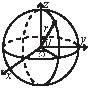
\includegraphics[width=25mm]{../code/sphericalCoordinates}}
\[\begin{array}{cc}
x = r\sin\theta\cos\phi & r = \sqrt{x^2+y^2+z^2}\\
y = r\sin\theta\sin\phi & \theta = \textrm{acos}(z/\sqrt{x^2+y^2+z^2})\\
z = r\cos\theta & \phi = \textrm{atan2}(y,x)
\end{array}\]

\subsection{Sums}
  1^2 + 2^2 + 3^2 + \dots + n^2 &= \frac{n(2n+1)(n+1)}{6} \\
  1^3 + 2^3 + 3^3 + \dots + n^3 &= \frac{n^2(n+1)^2}{4} \\
  1^4 + 2^4 + 3^4 + \dots + n^4 &= \frac{n(n+1)(2n+1)(3n^2 + 3n - 1)}{30} \\
  $\Scale[0.85]{ \sum\limits_{i=1}^{n} i^{m} = \frac{1}{m + 1}  \left[ (n + 1)^{m + 1} - 1 - \sum\limits_{i=1}^{n} \left((i+1)^{m+1} - i^{m+1} - (m + 1)i^{m}\right)\right]} $\\
  $\Scale[0.99]{\sum\limits_{i=1}^{n-1} i^{m} = \frac{1}{m + 1} \sum\limits_{k=0}^{m} { {m+1}\choose{k} } B_{k}n^{m + 1 - k}}$\\
  $\sum\limits_{k=0}^n kx^k = (x - (n+1)x^{n+1} + nx^{n+2})/(x-1)^2$


\subsection{Series}
$$e^x = 1+x+\frac{x^2}{2!}+\frac{x^3}{3!}+\dots,\,(-\infty<x<\infty)$$
$$\ln(1+x) = x-\frac{x^2}{2}+\frac{x^3}{3}-\frac{x^4}{4}+\dots,\,(-1<x\leq1)$$
$$\sqrt{1+x} = 1+\frac{x}{2}-\frac{x^2}{8}+\frac{2x^3}{32}-\frac{5x^4}{128}+\dots,\,(-1\leq x\leq1)$$
$$\sin x = x-\frac{x^3}{3!}+\frac{x^5}{5!}-\frac{x^7}{7!}+\dots,\,(-\infty<x<\infty)$$
$$\cos x = 1-\frac{x^2}{2!}+\frac{x^4}{4!}-\frac{x^6}{6!}+\dots,\,(-\infty<x<\infty)$$
$$(x + a)^{-n} = \sum\limits_{k=0}^{\infty} (-1)^{k} { {n + k - 1}\choose{k}} x^{k}a^{-n-k}$$

\subsection{Pythagorean Triples}
 The Pythagorean triples are uniquely generated by
 \[ a=k\cdot (m^{2}-n^{2}),\ \,b=k\cdot (2mn),\ \,c=k\cdot (m^{2}+n^{2}), \]
 with $m > n > 0$, $k > 0$, $m \bot n$, and either $m$ or $n$ even.


\subsection{Number Theory}
\subsubsection{Primes}
  $p=962592769$ is such that $2^{21} \mid p-1$, which may be useful. For hashing
  use 970592641 (31-bit number), 31443539979727 (45-bit), 3006703054056749
  (52-bit). There are 78498 primes less than 1\,000\,000.

  Primitive roots exist modulo any prime power $p^a$, except for $p = 2, a > 2$, and there are $\phi(\phi(p^a))$ many.
  For $p = 2, a > 2$, the group $\mathbb Z_{2^a}^\times$ is instead isomorphic to $\mathbb Z_2 \times \mathbb Z_{2^{a-2}}$.

\subsubsection{Estimates}
  $\sum_{d|n} d = O(n \log \log n)$.

  The number of divisors of $n$ is at most around 100 for $n < 5e4$, 500 for $n < 1e7$, 2000 for $n < 1e10$, 200\,000 for $n < 1e19$.

\subsubsection{Perfect numbers}  $n>1$ is called perfect if it equals
sum of its proper divisors and $1$.  Even $n$ is perfect iff $n = 2^{p-1} (2^p - 1)$
and $2^p - 1$ is prime (Mersenne's). No odd perfect numbers are yet found.

\subsubsection{Carmichael numbers}
A positive composite $n$ is a Carmichael number
($a^{n-1} \equiv 1 \pmod{n}$ for all $a$: $\gcd(a,n)=1$),
iff $n$ is square-free, and for all prime divisors $p$ of $n$, $p-1$ divides $n-1$.

\subsubsection{Mobius function}
$\mu(1) = 1$. $\mu(n) = 0$, if $n$ is not squarefree.
$\mu(n) = (-1)^s$, if $n$ is the product of $s$ distinct primes.
Let $f$, $F$ be functions on positive integers.
If for all $n \in N$, $F(n)=\sum_{d|n} f(d)$, then $f(n) = \sum_{d|n} \mu(d) F(\frac{n}{d})$,
and vice versa. \quad
$\phi(n) = \sum_{d|n} \mu(d) \frac{n}{d}$.
\quad $\sum_{d|n} \mu(d) = 1$. \\
If $f$ is multiplicative, then $\sum_{d|n} \mu(d) f(d) = \prod_{p|n}(1-f(p))$,
$\sum_{d|n} \mu(d)^2 f(d) = \prod_{p|n} (1+f(p))$.

\subsubsection{Legendre symbol} If $p$ is an odd prime, $a \in {\mathbb Z}$, then
$\left(\frac{a}{p}\right)$ equals $0$, if $p | a$; $1$ if $a$ is a quadratic
residue modulo $p$; and $-1$ otherwise.
Euler's criterion:
$\left(\frac{a}{p}\right)=a^{\left(\frac{p-1}{2}\right)} \pmod p$. \\
%$\left(\frac{a}{p}\right) \left(\frac{b}{p}\right) = \left(\frac{ab}{p}\right)$
%Law of Quadratic Reciprocity: for any distinct odd primes $p$ and $q$,
%$\left(\frac{p}{q}\right) \left(\frac{q}{p}\right) = (-1)^{\frac{p-1}{2} \cdot \frac{q-1}{2}}$
\subsubsection{Jacobi symbol}  %Generalization of Legendre's symbol to any odd modulus. \\
If $n=p_1^{a_1} \cdots p_k^{a_k}$ is odd, then
$\left(\frac{a}{n}\right) = \prod_{i=1}^k \left(\frac{a}{p_i}\right)^{k_i}$.

%\subsubsection{Kronecker symbol}
%Let $a$ be a positive integer, which is not a perfect square and
%$a \equiv 0$ or $1 {\pmod 4}$. \\
%$\left(\frac{a}{2}\right) = \{ 1$, if $a \equiv 1 {\pmod 8}$;
%$-1$, if $a \equiv 5 {\pmod 8} \}$. \\
%$\left(\frac{a}{n}\right) = \prod_{j=1}^k p_j^{k_j}$,
%if gcd$(a,n) \ne 1$ and $n=\prod p_i^{k_i}$.
%$\left(\frac{a}{n}\right)$ equals Jacobi symbol otherwise.

\subsubsection{Primitive roots}  If the order of $g$ modulo $m$ (min $n>0$:
$g^n \equiv 1 \pmod{m}$) is $\phi(m)$, then $g$ is called a primitive root.
If $Z_m$ has a primitive root, then it has $\phi(\phi(m))$ distinct primitive
roots. $Z_m$ has a primitive root iff $m$ is one of $2$, $4$,
$p^k$, $2p^k$, where $p$ is an odd prime.
If $Z_m$ has a primitive root $g$, then for all $a$ coprime to $m$,
there exists unique integer $i=\text{ind}_g(a)$ modulo $\phi(m)$,
such that $g^i \equiv a \pmod{m}$.
$\text{ind}_g(a)$ has logarithm-like properties:
$\text{ind}(1) = 0$, $\text{ind}(ab) = \text{ind}(a) + \text{ind}(b)$.

If $p$ is prime and $a$ is not divisible by $p$, then congruence
$x^n \equiv a \pmod{p}$ has $\gcd(n, p-1)$ solutions if
$a^{(p-1)/\gcd(n,p-1)} \equiv 1 \pmod{p}$, and no solutions otherwise.
(Proof sketch: let $g$ be a primitive root, and
$g^i \equiv a \pmod{p}$, $g^u \equiv x \pmod{p}$.
$x^n \equiv a \pmod{p}$ iff $g^{nu} \equiv g^i \pmod{p}$ iff $nu \equiv i \pmod{p}$.)

\subsubsection{Discrete logarithm problem}  Find $x$ from $a^x \equiv b \pmod{m}$.
Can be solved in $O(\sqrt{m})$ time and space with a meet-in-the-middle trick.
Let $n = \lceil \sqrt{m} \rceil$, and $x = ny - z$.
Equation becomes $a^{ny} \equiv b a^z \pmod{m}$.  Precompute all values that
the RHS can take for $z = 0, 1, \dots, n-1$, and brute force $y$ on the LHS,
each time checking whether there's a corresponding value for RHS.

\subsubsection{Pythagorean triples}  Integer solutions of $x^2 + y^2 = z^2$
All relatively prime triples are given by:
$x=2mn, y=m^2-n^2, z=m^2+n^2$ where $m>n, \gcd(m,n)=1$ and $m \not\equiv n \pmod{2}$.
All other triples are multiples of these.
Equation $x^2 + y^2 = 2z^2$ is equivalent to $(\frac{x+y}{2})^2 + (\frac{x-y}{2})^2 = z^2$.

\subsubsection{Postage stamps/McNuggets problem}  Let $a$, $b$ be relatively-prime integers.
There are exactly $\frac{1}{2}(a-1)(b-1)$ numbers \emph{not} of form $ax+by$ ($x,y \ge 0$),
and the largest is $(a-1)(b-1)-1 = ab - a - b$.

\subsubsection{Fermat's two-squares theorem}  Odd prime $p$ can be represented
as a sum of two squares iff $p \equiv 1 {\pmod 4}$.
A product of two sums of two squares is a sum of two squares.
Thus, $n$ is a sum of two squares iff every prime of
form $p=4k+3$ occurs an even number of times in $n$'s factorization.

% }}}

\subsection{Permutations}
  \subsubsection{Factorial}
    \begin{center}
\begin{tabular}{l}
\begin{tabular}{c|c@{\ }c@{\ }c@{\ }c@{\ }c@{\ }c@{\ }c@{\ }c@{\ }c@{\ }c}
$n$  & 1 & 2 & 3 & 4  & 5   & 6   & 7    & 8     & 9      & 10\\
\hline
$n!$ & 1 & 2 & 6 & 24 & 120 & 720 & 5040 & 40320 & 362880 & 3628800\\
\end{tabular}\\
\begin{tabular}{c|c@{\ }c@{\ }c@{\ }c@{\ }c@{\ }c@{\ }c@{\ }c@{\ }c@{\ }c}
$n$  & 11    & 12    & 13    & 14     & 15     & 16     & 17\\
\hline
$n!$ & 4.0e7 & 4.8e8 & 6.2e9 & 8.7e10 & 1.3e12 & 2.1e13 & 3.6e14\\
\end{tabular}\\
\begin{tabular}{c|c@{\ }c@{\ }c@{\ }c@{\ }c@{\ }c@{\ }c@{\ }c@{\ }c@{\ }c}
$n$  & 20   & 25   & 30   & 40   & 50   & 100   & 150   & 171\\
\hline
$n!$ & 2e18 & 2e25 & 3e32 & 8e47 & 3e64 & 9e157 & 6e262 & \scriptsize{$>$DBL\_MAX}\\
\end{tabular}
\end{tabular}
\end{center}


  \subsubsection{Cycles}
    Let $g_S(n)$ be the number of $n$-permutations whose cycle lengths all belong to the set $S$. Then
    $$\sum_{n=0} ^\infty g_S(n) \frac{x^n}{n!} = \exp\left(\sum_{n\in S} \frac{x^n} {n} \right)$$

  \subsubsection{Derangements}
    Permutations of a set such that none of the elements appear in their original position.
    \[ \mkern-2mu D(n) = (n-1)(D(n-1)+D(n-2)) = n D(n-1)+(-1)^n = \left\lfloor\frac{n!}{e}\right\rceil \]

  \subsubsection{Burnside's lemma}
    Given a group $G$ of symmetries and a set $X$, the number of elements of $X$ \emph{up to symmetry} equals
     \[ {\frac {1}{|G|}}\sum _{{g\in G}}|X^{g}|, \]
     where $X^{g}$ are the elements fixed by $g$ ($g.x = x$).

     If $f(n)$ counts ``configurations'' (of some sort) of length $n$, we can ignore rotational symmetry using $G = \mathbb Z_n$ to get
     \[ g(n) = \frac 1 n \sum_{k=0}^{n-1}{f(\text{gcd}(n, k))} = \frac 1 n \sum_{k|n}{f(k)\phi(n/k)} \]

\subsection{Partitions and subsets}
  \subsubsection{Partition function}
    Number of ways of writing $n$ as a sum of positive integers, disregarding the order of the summands.
    \[ p(0) = 1,\ p(n) = \sum_{k \in \mathbb Z \setminus \{0\}}{(-1)^{k+1} p(n - k(3k-1) / 2)} \]
    \[ p(n) \sim 0.145 / n \cdot \exp(2.56 \sqrt{n}) \]

    \begin{center}
    \begin{tabular}{c|c@{\ }c@{\ }c@{\ }c@{\ }c@{\ }c@{\ }c@{\ }c@{\ }c@{\ }c@{\ }c@{\ }c@{\ }c}
      $n$    & 0 & 1 & 2 & 3 & 4 & 5 & 6  & 7  & 8  & 9  & 20  & 50  & 100 \\ \hline
      $p(n)$ & 1 & 1 & 2 & 3 & 5 & 7 & 11 & 15 & 22 & 30 & 627 & $\mathtt{\sim}$2e5 & $\mathtt{\sim}$2e8 \\
    \end{tabular}
    \end{center}

\subsection{General purpose numbers}
  \subsubsection{Stirling numbers of the first kind}
    Number of permutations on $n$ items with $k$ cycles.
    \begin{align*}
      &c(n,k) = c(n-1,k-1) + (n-1) c(n-1,k),\ c(0,0) = 1 \\
      &\textstyle \sum_{k=0}^n c(n,k)x^k = x(x+1) \dots (x+n-1)
    \end{align*}
    $c(8,k) = 8, 0, 5040, 13068, 13132, 6769, 1960, 322, 28, 1$ \\
    $c(n,2) = 0, 0, 1, 3, 11, 50, 274, 1764, 13068, 109584, \dots$

  \subsubsection{Eulerian numbers}
    Number of permutations $\pi \in S_n$ in which exactly $k$ elements are greater than the previous element. $k$ $j$:s s.t. $\pi(j)>\pi(j+1)$, $k+1$ $j$:s s.t. $\pi(j)\geq j$, $k$ $j$:s s.t. $\pi(j)>j$.
    $$E(n,k) = (n-k)E(n-1,k-1) + (k+1)E(n-1,k)$$
    $$E(n,0) = E(n,n-1) = 1$$
    $$E(n,k) = \sum_{j=0}^k(-1)^j\binom{n+1}{j}(k+1-j)^n$$

  \subsubsection{Stirling numbers of the second kind}
    Partitions of $n$ distinct elements into exactly $k$ groups.
    $$S(n,k) = S(n-1,k-1) + k S(n-1,k)$$
    $$S(n,1) = S(n,n) = 1$$
    $$S(n,k) = \frac{1}{k!}\sum_{j=0}^k (-1)^{k-j}\binom{k}{j}j^n$$

  \subsubsection{Bell numbers}
    Total number of partitions of $n$ distinct elements. $B(n) =$
    $1, 1, 2, 5, 15, 52, 203, 877, 4140, 21147, \dots$. For $p$ prime,
    \[ B(p^m+n)\equiv mB(n)+B(n+1) \pmod{p} \]

  \subsubsection{Bernoulli numbers}
  $\Scale[.95]{\sum\limits_{j=0}^m {m+1 \choose j} B_j = 0$.
  \quad $B_0=1$, $B_1=-\frac{1}{2}$. $B_n=0$, for all odd $n \ne 1}$.

  \subsubsection{Catalan numbers}
    \[ C_n=\frac{1}{n+1}\binom{2n}{n}= \binom{2n}{n}-\binom{2n}{n+1} = \frac{(2n)!}{(n+1)!n!} \]
    \[ C_0=1,\ C_{n+1} = \frac{2(2n+1)}{n+2}C_n,\ C_{n+1}=\sum C_iC_{n-i} \]
    ${C_n = 1, 1, 2, 5, 14, 42, 132, 429, 1430, 4862, 16796, 58786, \dots}$
    \begin{itemize}[noitemsep]
      \item sub-diagonal monotone paths in an $n\times n$ grid.
      \item strings with $n$ pairs of parenthesis, correctly nested.
      \item binary trees with with $n+1$ leaves (0 or 2 children).
      \item ordered trees with $n+1$ vertices.
      \item ways a convex polygon with $n+2$ sides can be cut into triangles by connecting vertices with straight lines.
      \item permutations of $[n]$ with no 3-term increasing subseq.
    \end{itemize}

\subsection{Inequalities}
\subsubsection{Titu's Lemma}
For positive reals $a_1, a_2, \ldots, a_n$ and $b_1, b_2, \ldots, b_n$,
$$\frac{{a_1}^2}{b_1} + \frac{{a_2}^2}{b_2} + \ldots + \frac{{a_n}^2}{b_n} \geq \frac{{a_1 + a_2 + \ldots + a_n}^2}{b_1 + b_2 + \ldots + b_n}$$
Equality holds if and only if $ a_i = kb_i$ for a non-zero real constant $k$.
\subsection{Games}

\subsubsection{Grundy numbers}
For a two-player, normal-play (last to move wins) game on a graph $(V,E)$:
$G(x) = \mbox{mex}(\{ G(y) : (x, y) \in E \})$,
where $\mbox{mex}(S) = \min \{ n \ge 0: n \not\in S \}$.
$x$ is losing iff $G(x) = 0$.

\subsubsection{Sums of games}

\vspace{-1mm}
\begin{itemize}
  \item
    \emph{Player chooses a game and makes a move in it}
    Grundy number of a position is xor of grundy numbers of positions in summed games.
    \vspace{-1mm}
  \item
    \emph{Player chooses a non-empty subset of games (possibly, all) and makes moves in all of them}
    A position is losing iff each game is in a losing position.
  \vspace{-1mm}
  \item
    \emph{Player chooses a proper subset of games (not empty and not all),
        and makes moves in all chosen ones.}
    A position is losing iff grundy numbers of all games are equal.
    \vspace{-1mm}
  \item
    \emph{Player must move in all games, and loses if can't move in some game}
    A position is losing if any of the games is in a losing position.
\end{itemize}

\subsubsection{Mis\`{e}re Nim}
A position with pile sizes $a_1, a_2, \dots, a_n \ge 1$,
not all equal to $1$, is losing iff $a_1 \oplus a_2 \oplus \dots \oplus a_n = 0$
(like in normal nim.)
A position with $n$ piles of size $1$ is losing iff $n$ is \emph{odd}.
\subsection{NumberTheory}
\begin{equation}
\sum_{k=1}^n \frac{1}{\operatorname{gcd}(k, n)}=\sum_{d \mid n} \frac{1}{d} \cdot \phi\left(\frac{n}{d}\right)=\frac{1}{n} \sum_{d \mid n} d \cdot \phi(d) \\
\end{equation}
\begin{equation}
\sum_{k=1}^n \frac{k}{\operatorname{gcd}(k, n)}=\frac{n}{2} \cdot \frac{1}{n} \cdot \sum_{d \mid n} d \cdot \phi(d) \\
\end{equation}
\begin{equation}
\sum_{k=1}^n \frac{n}{\operatorname{gcd}(k, n)}=2 * \sum_{k=1}^n \frac{k}{\operatorname{gcd}(k, n)}-1, \text { for, } n>1
\end{equation}
\begin{equation}
\sum_{i=1}^n \sum_{j=1}^n[\operatorname{gcd}(i, j)=1]=\sum_{d=1}^n \mu(d)\left\lfloor\frac{n}{d}\right\rfloor^2 \\
\end{equation}
\begin{equation}
\sum_{i=1}^n \sum_{j=1}^n \operatorname{gcd}(i, j)=\sum_{d=1}^n \phi(d)\left\lfloor\frac{n}{d}\right\rfloor^2 \\
\end{equation}
\begin{equation}
\sum_{i=1}^n \sum_{j=1}^n i \cdot j[\operatorname{gcd}(i, j)=1]=\sum_{i=1}^n \phi(i) i^2 \\
\end{equation}
\begin{equation}
\sum_{i=1}^n \sum_{j=1}^n \operatorname{lcm}(i, j)=\sum_{l=1}^n\left(\frac{\left(1+\left\lfloor\frac{n}{l}\right\rfloor\right)\left(\left\lfloor\frac{n}{l}\right\rfloor\right)}{2}\right)^2=\sum_{d \mid l} \mu(d) l d
\end{equation}
\section{String}
\subsection{aho\_corasick}
\begin{minted}[
    breaklines = true,
    breakanywhere = true,
    frame=lines,    
    fontfamily=tt,
    linenos=false,
    numberblanklines=true,
    numbersep=2pt,
    gobble=0,
    framerule=1pt,
    framesep=1mm,
    funcnamehighlighting=true,
    tabsize=1,
    obeytabs=false,
    mathescape=false
    samepage=false, %with this setting you can force the list to appear on the same page
    showspaces=false,
    showtabs =false,
    texcl=false
]{C++}

using namespace std;

const int N = ?;
const int A = ?;

struct AC {
  int nd, pt;

  int next[N][A], link[N], out_link[N], cnt[N], ans[N];
  vector <int> ed[N], out[N];

  AC(): nd(0), pt(0) { node(); }

  int node() {
    memset(next[nd], 0, sizeof next[nd]);
    link[nd] = out_link[nd] = cnt[nd] = 0;
    ed[nd].clear(), out[nd].clear();
    return nd++;
  }

  void clear() {
    nd = pt = 0;
    node();
  }

  inline int get(char c) { return c - 'a'; }

  void insert(const string &T) {
    int u = 0;
    for (char c : T) {
      if (!next[u][get(c)]) next[u][get(c)] = node();
      u = next[u][get(c)];
    }
    ans[pt] = 0;
    out[u].push_back(pt++);
  }

  void build() {
    queue <int> q;
    for (q.push(0); !q.empty(); ) {
      int u = q.front();
      q.pop();
      for (int c = 0; c < A; ++c) {
        int v = next[u][c];
        if (!v) next[u][c] = next[link[u]][c];
        else {
          link[v] = u ? next[link[u]][c] : 0;
          out_link[v] = out[link[v]].empty() ? out_link[link[v]] : link[v];
          ed[link[v]].push_back(v);
          q.push(v);
        }
      }
    }
  }

  void dfs(int s) {
    for(int x : ed[s]) dfs(x), cnt[s] += cnt[x];
    for(int e : out[s]) ans[e] = cnt[s];
  }

  void traverse(const string &S) {
    int u = 0;
    for (char c : S) {
      u = next[u][get(c)];
      cnt[u]++;
    }
    dfs(0);
  }
};

char str[1000010], pat[505];

int main() {
  //    freopen("in.txt","r",stdin);
  AC aho;
  int t,T;
  scanf("%d",&T);
  for(int t=1;t<=T;t++) {
    int n;
    scanf("%d",&n);
    scanf("%s",str);
    for(int i=1;i<=n;i++) {
      scanf("%s",pat);
      aho.insert(pat);
    }
    aho.build();
    aho.traverse(str);
    printf("Case %d:\n",t);
    for(int i=0;i<n;i++) {
      printf("%d\n",aho.ans[i]);
    }
    aho.clear();
  }
  return 0;
}
\end{minted}

\subsection{hash}
\begin{minted}[
    breaklines = true,
    breakanywhere = true,
    frame=lines,    
    fontfamily=tt,
    linenos=false,
    numberblanklines=true,
    numbersep=2pt,
    gobble=0,
    framerule=1pt,
    framesep=1mm,
    funcnamehighlighting=true,
    tabsize=1,
    obeytabs=false,
    mathescape=false
    samepage=false, %with this setting you can force the list to appear on the same page
    showspaces=false,
    showtabs =false,
    texcl=false
]{C++}

struct Hash {
  struct base {
    string s; int b, mod;
    vector<int> hash, p;
    void init(string &_s, int _b, int _mod) { // b > 26, prime.
      s = _s; b = _b, mod = _mod;
      hash.resize(s.size());
      p.resize(s.size());
      hash[0] = s[0] - 'A' + 1; p[0] = 1;
      for(int i = 1; i < s.size(); ++i) {
        hash[i] = (ll) hash[i - 1] * b % mod;
        hash[i] += s[i] - 'A' + 1;
        if(hash[i] >= mod) hash[i] -= mod;
        p[i] = (ll) p[i - 1] * b % mod;
      }
    }
    int get(int l, int r) {
      int ret = hash[r];
      if(l) ret -= (ll) hash[l - 1] * p[r - l + 1] % mod;
      if(ret < 0) ret += mod;
      return ret;
    }
  } h[2];
  void init(string &s) {
    h[0].init(s, 29, 1e9+7);
    h[1].init(s, 31, 1e9+9);
  }
  pair<int, int> get(int l, int r) {
    return { h[0].get(l, r), h[1].get(l, r) };
  }
} H;
\end{minted}

\subsection{hash\_segtree}
\begin{minted}[
    breaklines = true,
    breakanywhere = true,
    frame=lines,    
    fontfamily=tt,
    linenos=false,
    numberblanklines=true,
    numbersep=2pt,
    gobble=0,
    framerule=1pt,
    framesep=1mm,
    funcnamehighlighting=true,
    tabsize=1,
    obeytabs=false,
    mathescape=false
    samepage=false, %with this setting you can force the list to appear on the same page
    showspaces=false,
    showtabs =false,
    texcl=false
]{C++}

#define INVALID_CHAR        -1

namespace strhash {
  int n;
  const int MAX = 100010;
  int ara[MAX];
  const int MOD[] = {1067737007, 1069815139};
  const int BASE[] = {982451653, 984516781};


  int BP[2][MAX], CUM[2][MAX];

  void init(char *str) {
    n = strlen(str);
    for(int i=0;i<n;i++) ara[i] = str[i]-'0'+1;
  }

  void precal() {
    BP[0][0] = BP[1][0] = 1;
    CUM[0][0] = CUM[1][0] = 1;
    for(int i=1;i<MAX;i++) {
      BP[0][i] = ( BP[0][i-1] * (long long) BASE[0] ) % MOD[0];
      BP[1][i] = ( BP[1][i-1] * (long long) BASE[1] ) % MOD[1];

      CUM[0][i] = ( CUM[0][i-1] + (long long) BP[0][i] ) % MOD[0];
      CUM[1][i] = ( CUM[1][i-1] + (long long) BP[1][i] ) % MOD[1];
    }
  }

  struct node {
    int sz;
    int h[2];
    node() {}
  } tree[4*MAX];

  int lazy[4*MAX];

  inline void lazyUpdate(int n,int st,int ed) {
    if(lazy[n]!=INVALID_CHAR){

      tree[n].h[0] = (lazy[n] * (long long) CUM[0][ed-st]) % MOD[0];
      tree[n].h[1] = (lazy[n] * (long long) CUM[1][ed-st]) % MOD[1];

      if(st!=ed){
        lazy[2*n] = lazy[n];
        lazy[2*n+1] = lazy[n];
      }
      lazy[n] = INVALID_CHAR;
    }
  }

  inline node Merge(node a,node b) {
    node ret;

    ret.h[0] = ( ( a.h[0] * (long long) BP[0][b.sz] ) + b.h[0] ) % MOD[0];
    ret.h[1] = ( ( a.h[1] * (long long) BP[1][b.sz] ) + b.h[1] ) % MOD[1];

    ret.sz = a.sz + b.sz;

    return ret;
  }

  inline void build(int n,int st,int ed) {
    lazy[n] = INVALID_CHAR;
    if(st==ed) {
      tree[n].h[0] = tree[n].h[1] = ara[st];
      tree[n].sz = 1;
      return;
    }
    int mid = (st+ed)>>1;
    build(n+n,st,mid);
    build(n+n+1,mid+1,ed);

    tree[n] = Merge(tree[n+n],tree[n+n+1]);
  }


  inline void update(int n,int st,int ed,int i,int j,int v) {
    lazyUpdate(n,st,ed);
    if(st>j or ed<i) return;
    if(st>=i and ed<=j) {
      lazy[n] = v;
      lazyUpdate(n,st,ed);
      return;
    }

    int mid = (st+ed)>>1;
    update(n+n,st,mid,i,j,v);
    update(n+n+1,mid+1,ed,i,j,v);

    tree[n] = Merge(tree[n+n],tree[n+n+1]);
  }

  inline node query(int n,int st,int ed,int i,int j){
    lazyUpdate(n,st,ed);
    if(st>=i and ed<=j) return tree[n];
    int mid = (st+ed)/2;
    if(mid<i) return query(n+n+1,mid+1,ed,i,j);
    else if(mid>=j) return query(n+n,st,mid,i,j);
    else return Merge(query(n+n,st,mid,i,j),query(n+n+1,mid+1,ed,i,j));
  }
}
\end{minted}

\subsection{kmp}
\begin{minted}[
    breaklines = true,
    breakanywhere = true,
    frame=lines,    
    fontfamily=tt,
    linenos=false,
    numberblanklines=true,
    numbersep=2pt,
    gobble=0,
    framerule=1pt,
    framesep=1mm,
    funcnamehighlighting=true,
    tabsize=1,
    obeytabs=false,
    mathescape=false
    samepage=false, %with this setting you can force the list to appear on the same page
    showspaces=false,
    showtabs =false,
    texcl=false
]{C++}

// returns the longest proper prefix array of pattern p
// where lps[i]=longest proper prefix which is also suffix of p[0...i]
vector<int> build_lps(string p) {
  int sz = p.size();
  vector<int> lps;
  lps.assign(sz + 1, 0);
  int j = 0;
  lps[0] = 0;
  for(int i = 1; i < sz; i++) {
    while(j >= 0 && p[i] != p[j]) {
      if(j >= 1) j = lps[j - 1];
      else j = -1;
    }
    j++;
    lps[i] = j;
  }
  return lps;
}
vector<int>ans;
// returns matches in vector ans in 0-indexed
void kmp(vector<int> lps, string s, string p) {
  int psz = p.size(), sz = s.size();
  int j = 0;
  for(int i = 0; i < sz; i++) {
    while(j >= 0 && p[j] != s[i])
      if(j >= 1) j = lps[j - 1];
      else j = -1;
    j++;
    if(j == psz) {
      j = lps[j - 1];
      // pattern found in string s at position i-psz+1
      ans.push_back(i - psz + 1);
    }
    // after each loop we have j=longest common suffix of s[0..i] which is also prefix of p
  }
}
\end{minted}

\subsection{manachar}
\begin{minted}[
    breaklines = true,
    breakanywhere = true,
    frame=lines,    
    fontfamily=tt,
    linenos=false,
    numberblanklines=true,
    numbersep=2pt,
    gobble=0,
    framerule=1pt,
    framesep=1mm,
    funcnamehighlighting=true,
    tabsize=1,
    obeytabs=false,
    mathescape=false
    samepage=false, %with this setting you can force the list to appear on the same page
    showspaces=false,
    showtabs =false,
    texcl=false
]{C++}

vector<int> d1(n);  // maximum odd length palindrome centered at i
                    // here d1[i]=the palindrome has d1[i]-1 right characters from i
                    // e.g. for aba, d1[1]=2;
for (int i = 0, l = 0, r = -1; i < n; i++) {
  int k = (i > r) ? 1 : min(d1[l + r - i], r - i);
  while (0 <= i - k && i + k < n && s[i - k] == s[i + k]) {
    k++;
  }
  d1[i] = k--;
  if (i + k > r) {
    l = i - k;
    r = i + k;
  }
}
vector<int> d2(n);  // maximum even length palindrome centered at i
                    // here d2[i]=the palindrome has d2[i]-1 right characters from i
                    // e.g. for abba, d2[2]=2;
for (int i = 0, l = 0, r = -1; i < n; i++) {
  int k = (i > r) ? 0 : min(d2[l + r - i + 1], r - i + 1);
  while (0 <= i - k - 1 && i + k < n && s[i - k - 1] == s[i + k]) {
    k++;
  }
  d2[i] = k--;
  if (i + k > r) {
    l = i - k - 1;
    r = i + k ;
  }
}
\end{minted}

\subsection{palindromic\_tree}
\begin{minted}[
    breaklines = true,
    breakanywhere = true,
    frame=lines,    
    fontfamily=tt,
    linenos=false,
    numberblanklines=true,
    numbersep=2pt,
    gobble=0,
    framerule=1pt,
    framesep=1mm,
    funcnamehighlighting=true,
    tabsize=1,
    obeytabs=false,
    mathescape=false
    samepage=false, %with this setting you can force the list to appear on the same page
    showspaces=false,
    showtabs =false,
    texcl=false
]{C++}

const int A = 26;
const int N = 300010;

char s[N]; long long ans;
int last, ptr, nxt[N][A], link[N], len[N], occ[N];

void feed (int at) {
  while (s[at - len[last] - 1] != s[at]) last = link[last];
  int ch = s[at] - 'a', temp = link[last];
  while (s[at - len[temp] - 1] != s[at]) temp = link[temp];
  if (!nxt[last][ch]) {
    nxt[last][ch] = ++ptr, len[ptr] = len[last] + 2;
    link[ptr] = len[ptr] == 1 ? 2 : nxt[temp][ch];
  }
  last = nxt[last][ch], ++occ[last];
}

int main() {
  len[1] = -1, len[2] = 0, link[1] = link[2] = 1, last = ptr = 2;
  scanf("%s", s + 1);
  for (int i = 1, n = strlen(s + 1); i <= n; ++i) feed(i);
  for (int i = ptr; i > 2; --i) ans = max(ans, len[i] * 1LL * occ[i]), occ[link[i]] += occ[i];
  printf("%lld\n", ans);
  return 0;
}
\end{minted}

\subsection{persistant\_trie}
\begin{minted}[
    breaklines = true,
    breakanywhere = true,
    frame=lines,    
    fontfamily=tt,
    linenos=false,
    numberblanklines=true,
    numbersep=2pt,
    gobble=0,
    framerule=1pt,
    framesep=1mm,
    funcnamehighlighting=true,
    tabsize=1,
    obeytabs=false,
    mathescape=false
    samepage=false, %with this setting you can force the list to appear on the same page
    showspaces=false,
    showtabs =false,
    texcl=false
]{C++}

const int MAX = 200010;
const int B = 19;
int root[MAX], ptr = 0;

struct node {
  int ara[2], sum;
  node() {}
} tree[ MAX * (B+1) ];

void insert(int prevnode, int &curRoot, int val) {
  curRoot = ++ptr;
  int curnode = curRoot;
  for(int i = B; i >= 0; i--) {
    bool bit = val & (1 << i);
    tree[curnode] = tree[prevnode];
    tree[curnode].ara[bit] = ++ptr;
    tree[curnode].sum += 1;
    prevnode = tree[prevnode].ara[bit];
    curnode = tree[curnode].ara[bit];
  }
  tree[curnode] = tree[prevnode];
  tree[curnode].sum += 1;
}

int find_xor_max(int prevnode, int curnode, int x) {
  int ans = 0;
  for(int i = B; i >= 0; i--) {
    bool bit = x & (1 << i);
    if(tree[tree[curnode].ara[bit ^ 1]].sum > tree[tree[prevnode].ara[bit ^ 1]].sum) {
      curnode = tree[curnode].ara[bit ^ 1];
      prevnode = tree[prevnode].ara[bit ^ 1];
      ans = ans | (1 << i);
    }
    else {
      curnode = tree[curnode].ara[bit];
      prevnode = tree[prevnode].ara[bit];
    }
  }
  return ans;
}

void solve() {
  int n, q, L, R, K;
  cin >> n;
  for(int i=1;i<=n;i++) cin >> ara[i];

  for(int i=1;i<=q;i++) {
    cin >> L >> R >> K;
    cout << find_xor_max(root[L-1],root[R],K) << endl;
  }
}
\end{minted}

\subsection{suffix\_array}
\begin{minted}[
    breaklines = true,
    breakanywhere = true,
    frame=lines,    
    fontfamily=tt,
    linenos=false,
    numberblanklines=true,
    numbersep=2pt,
    gobble=0,
    framerule=1pt,
    framesep=1mm,
    funcnamehighlighting=true,
    tabsize=1,
    obeytabs=false,
    mathescape=false
    samepage=false, %with this setting you can force the list to appear on the same page
    showspaces=false,
    showtabs =false,
    texcl=false
]{C++}

// Everything is 0-indexed
char s[N]; // Suffix array will be built for this string
int SA[N], iSA[N]; // SA is the suffix array, iSA[i] stores the rank of the i'th suffix
int cnt[N], nxt[N]; // Internal stuff
bool bh[N], b2h[N]; // Internal stuff
int lcp[N]; // Stores lcp of SA[i] and SA[i + 1]; lcp[n - 1] = 0
int lcpSparse[LOGN][N]; // lcpSparse[i][j] = min(lcp[j], ..., lcp[j - 1 + (1 << i)])

void buildSA(int n) {
  for (int i = 0; i < n; i++) SA[i] = i;
  sort(SA, SA + n, [](int i, int j) { return s[i] < s[j]; });

  for (int i = 0; i < n; i++) {
    bh[i] = i == 0 || s[SA[i]] != s[SA[i - 1]];
    b2h[i] = 0;
  }

  for (int h = 1; h < n; h <<= 1) {
    int tot = 0;
    for (int i = 0, j; i < n; i = j) {
      j = i + 1;
      while (j < n && !bh[j]) j++;
      nxt[i] = j; tot++;
    } if (tot == n) break;

    for (int i = 0; i < n; i = nxt[i]) {
      for (int j = i; j < nxt[i]; j++) iSA[SA[j]] = i;
      cnt[i] = 0;
    }

    cnt[iSA[n - h]]++;
    b2h[iSA[n - h]] = 1;
    for (int i = 0; i < n; i = nxt[i]) {
      for (int j = i; j < nxt[i]; j++) {
        int s = SA[j] - h;
        if (s < 0) continue;
        int head = iSA[s];
        iSA[s] = head + cnt[head]++;
        b2h[iSA[s]] = 1;
      }
      for (int j = i; j < nxt[i]; j++) {
        int s = SA[j] - h;
        if (s < 0 || !b2h[iSA[s]]) continue;
        for (int k = iSA[s] + 1; !bh[k] && b2h[k]; k++) b2h[k] = 0;
      }
    }
    for (int i = 0; i < n; i++) {
      SA[iSA[i]] = i;
      bh[i] |= b2h[i];
    }
  }
  for (int i = 0; i < n; i++) iSA[SA[i]] = i;
}

void buildLCP(int n) {
  for (int i = 0, k = 0; i < n; i++) {
    if (iSA[i] == n - 1) {
      k = 0;
      lcp[n - 1] = 0;
      continue;
    }
    int j = SA[iSA[i] + 1];
    while (i + k < n && j + k < n && s[i + k] == s[j + k]) k++;
    lcp[iSA[i]] = k;
    if (k) k--;
  }
}

void buildLCPSparse(int n) {
  for (int i = 0; i < n; i++) lcpSparse[0][i] = lcp[i];
  for (int i = 1; i < LOGN; i++) {
    for (int j = 0; j < n; j++) {
      lcpSparse[i][j] = min(lcpSparse[i - 1][j], lcpSparse[i - 1][min(n - 1, j + (1 << (i - 1)))]);
    }
  }
}

pair<int, int> minLCPRange(int n, int from, int minLCP) {
  int r = from;
  for (int i = LOGN - 1; i >= 0; i--) {
    int jump = 1 << i;
    if (r + jump < n and lcpSparse[i][r] >= minLCP) r += jump;
  }

  int l = from;
  for (int i = LOGN - 1; i >= 0; i--) {
    int jump = 1 << i;
    if (l - jump >= 0 and lcpSparse[i][l - jump] >= minLCP) l -= jump;
  }

  return make_pair(l, r);
}
\end{minted}

\subsection{suffix\_automata}
\begin{minted}[
    breaklines = true,
    breakanywhere = true,
    frame=lines,    
    fontfamily=tt,
    linenos=false,
    numberblanklines=true,
    numbersep=2pt,
    gobble=0,
    framerule=1pt,
    framesep=1mm,
    funcnamehighlighting=true,
    tabsize=1,
    obeytabs=false,
    mathescape=false
    samepage=false, %with this setting you can force the list to appear on the same page
    showspaces=false,
    showtabs =false,
    texcl=false
]{C++}

namespace sa{
  const int MAXN = 100005 << 1;
  const int MAXC = 26;

  char str[MAXN];

  int n, sz, last;
  int len[MAXN], link[MAXN], ed[MAXN][MAXC], cnt[MAXN];
  bool terminal[MAXN];
  vector <int> G[MAXN];

  void init() {
    SET(ed[0]);
    len[0] = 0, link[0] = -1, sz = 1, last = 0, terminal[0] = false;
  }

  inline int scale(char c) { return c-'a'; }

  void extend(char c) {
    int cur = sz++;

    terminal[cur] = false;
    cnt[cur] = 1;

    SET(ed[cur]);
    len[cur] = len[last] + 1;
    int p = last;
    while (p != -1 && ed[p][c]==-1) {
      ed[p][c] = cur;
      p = link[p];
    }
    if (p == -1) link[cur] = 0;
    else {
      int q = ed[p][c];
      if (len[p] + 1 == len[q]) link[cur] = q;
      else {
        int clone = sz++;
        len[clone] = len[p] + 1;
        memcpy(ed[clone],ed[q],sizeof(ed[q]));
        link[clone] = link[q];
        while (p != -1 && ed[p][c] == q) {
          ed[p][c] = clone;
          p = link[p];
        }
        link[q] = link[cur] = clone;

        cnt[clone] = 0;
        terminal[clone] = false;
      }
    }
    last = cur;
  }

  void dfs(int s) {
    for(auto x : G[s]) dfs(x), cnt[s] += cnt[x];
  }

  void build() {
    init();
    int n = strlen(str);
    for(int i=0;i<n;i++) extend(scale(str[i]));

    for(int i=1;i<sz;i++) G[link[i]].pb(i);
    dfs(0);
    for(int i=0;i<sz;i++) G[i].clear();

    for(int i=last;i!=-1;i=link[i]) terminal[i] = true;
  }
}
\end{minted}

\subsection{trie}
\begin{minted}[
    breaklines = true,
    breakanywhere = true,
    frame=lines,    
    fontfamily=tt,
    linenos=false,
    numberblanklines=true,
    numbersep=2pt,
    gobble=0,
    framerule=1pt,
    framesep=1mm,
    funcnamehighlighting=true,
    tabsize=1,
    obeytabs=false,
    mathescape=false
    samepage=false, %with this setting you can force the list to appear on the same page
    showspaces=false,
    showtabs =false,
    texcl=false
]{C++}

#define N       200000
#define S       26

int root,now;
int nxt[N][S], cnt[N];

void init(){
  root = now = 1;
  CLR(nxt),CLR(cnt);
}

inline int scale(char ch) { return (ch - 'a'); }

inline void Insert(char s[],int sz){
  int cur = root, to;
  for(int i=0 ; i< sz ; i++){
    to = scale(s[i]) ;
    if( !nxt[cur][to] ) nxt[cur][to] = ++now;
    cur = nxt[cur][to];
  }
  cnt[cur]++;
}

inline bool Find(char s[],int sz){
  int cur = root, to;
  for(int i=0 ; i<sz ; i++){
    to = scale(s[i]) ;
    if( !nxt[cur][to] ) return false;
    cur = nxt[cur][to];
  }
  return (cnt[cur]!=0);
}

inline void Delete(char s[],int sz){
  int cur = root, to;
  for(int i=0 ; i<sz ; i++){
    to = scale(s[i]) ;
    cur = nxt[cur][to];
  }
  cnt[cur]--;
}
\end{minted}

\subsection{z\_algo}
\begin{minted}[
    breaklines = true,
    breakanywhere = true,
    frame=lines,    
    fontfamily=tt,
    linenos=false,
    numberblanklines=true,
    numbersep=2pt,
    gobble=0,
    framerule=1pt,
    framesep=1mm,
    funcnamehighlighting=true,
    tabsize=1,
    obeytabs=false,
    mathescape=false
    samepage=false, %with this setting you can force the list to appear on the same page
    showspaces=false,
    showtabs =false,
    texcl=false
]{C++}

const int N = 100010;

char s[N];
int t, n, z[N];

int main() {
  scanf("%s", s);
  n = strlen(s), z[0] = n;
  int L = 0, R = 0;
  for (int i = 1; i < n; ++i) {
    if (i > R) {
      L = R = i;
      while (R < n && s[R - L] == s[R]) ++R;
      z[i] = R - L; --R;
    } else {
      int k = i - L;
      if (z[k] < R - i + 1) z[i] = z[k];
      else {
        L = i;
        while (R < n && s[R - L] == s[R]) ++R;
        z[i] = R - L; --R;
      }
    }
  }
}
\end{minted}

\end{multicols}
\end{document}